\documentclass[a4paper,11pt]{ltjsarticle}
\usepackage[top=18mm,bottom=18mm,left=20mm,right=20mm]{geometry}
\usepackage{luatexja-fontspec}
\setmainjfont{Noto Serif CJK JP}[BoldFont=Noto Sans CJK JP Bold]
\setsansjfont{Noto Sans CJK JP}[BoldFont=Noto Sans CJK JP Bold]
\usepackage{amsmath,amssymb}
\usepackage{enumitem}
\usepackage{fancyhdr}
\usepackage{needspace}
\usepackage{multicol}
\usepackage[most]{tcolorbox}

\newtcolorbox{kai}{enhanced,breakable,colback=white,colframe=black,boxrule=0pt,
  borderline west={0.8pt}{0pt}{black},arc=0pt,left=8pt,right=0pt,top=2pt,bottom=2pt,
  before skip=3pt,after skip=8pt}

\pagestyle{fancy}
\fancyhf{}
\fancyhead[L]{\small\sffamily 数学Ⅰ・A 類題集}
\fancyhead[R]{\small\sffamily\leftmark}
\fancyfoot[C]{\small\thepage}
\renewcommand{\headrulewidth}{0.4pt}
\setlength{\parindent}{0pt}
\setlength{\parskip}{0.25em}
\setlist[enumerate,1]{label={(\arabic*)},leftmargin=2.2em,itemsep=2pt,topsep=2pt}

% 問題
\newcommand{\mon}[2]{\Needspace{7\baselineskip}\vspace{10pt}%
  {\sffamily\bfseries 類題 #1\quad #2\par}\vspace{2pt}\hrule\vspace{4pt}}
% 解答
\newcommand{\ans}[2]{\Needspace{5\baselineskip}\vspace{6pt}%
  {\sffamily\bfseries 類題 #1\quad #2}\par}
\newcommand{\point}[1]{\textsf{\bfseries ▶ #1}}
\newcommand{\rpt}[1]{0.\dot{#1}}

\usepackage{tikz}
\usetikzlibrary{calc,intersections}
\newcommand{\ax}[4]{\draw[->] (#1,0)--(#2,0) node[right]{\scriptsize $x$};
  \draw[->] (0,#3)--(0,#4) node[above]{\scriptsize $y$};
  \node[below left] at (0,0){\scriptsize O};}
\newcommand{\shou}[2]{\clearpage\markboth{#1\quad #2}{}%
  {\sffamily\bfseries\LARGE #1\quad #2\par}\vspace{2pt}\hrule height 1.2pt\vspace{4pt}}
\newcommand{\shouans}[2]{\Needspace{8\baselineskip}\vspace{10pt}\markboth{解答\quad #1\quad #2}{}%
  {\sffamily\bfseries\Large #1\quad #2\par}\vspace{2pt}\hrule height 0.8pt\vspace{2pt}}

\begin{document}
\thispagestyle{empty}
\begin{center}
\vspace*{50mm}
{\sffamily\bfseries\Huge 数学Ⅰ・A 類題集\par}
\vspace{8mm}
{\sffamily\Large 基礎問 類題1〜154\par}
\vspace{15mm}
\begin{minipage}{0.75\linewidth}\small
類題の番号は基礎問の番号に対応している．基礎問を学習したあと，同じ考え方で解けるかを確かめるのに使う．解答は後半にまとめてある．
\end{minipage}
\end{center}
\clearpage
\setcounter{page}{1}
\shou{第1章}{数と式}
\mon{1}{指数の計算}
次の式を簡単にせよ．
\[\text{(1)}\ \ 2^4\times2^3\qquad \text{(2)}\ \ (3^2)^3\qquad \text{(3)}\ \ x^3y\times xy^4\]
\[\text{(4)}\ \ 3x^2y\times2xy^3z\times5yz^2\qquad \text{(5)}\ \ (-3x^2y)^2\times(-2xy^2)^3\]

\mon{2}{整式の加減}
$A=2x^2-3x+1$，$B=x^2+5x-4$ のとき，$A+B$，$A-B$ を計算せよ．

\mon{3}{式の展開}
次の式を展開せよ．
\begin{enumerate}
\item $(x+y-z)(x-y-z)$
\item $(x^2-x+1)(2x^2-2x-3)$
\item $(x-1)(x+2)(x-3)(x+4)$
\item $(x-2)(x+2)(x^2+4)$
\item $(a-b-c)(a^2+b^2+c^2+ab-bc+ca)$
\end{enumerate}

\mon{4}{因数分解}
次の式を因数分解せよ．
\begin{multicols}{2}
\begin{enumerate}
\item $3x^3+2x^2-12x-8$
\item $xy-x-y+1$
\item $2a^3b+a^2b^2-3ab^3$
\item $x^4-10x^2+9$
\item $(x^2+x-5)(x^2+x-3)-3$
\item $xyz-xy-yz-zx+x+y+z-1$
\end{enumerate}
\end{multicols}

\mon{5}{対称式}
\begin{enumerate}
\item $x+y=3$，$xy=1$ のとき，次の値を求めよ．\\
(i)\ $x^2+y^2$\qquad (ii)\ $x^3+y^3$\qquad (iii)\ $x^4+y^4$
\item $x+\dfrac1x=3$ のとき，次の値を求めよ．\\
(i)\ $x^2+\dfrac1{x^2}$\qquad (ii)\ $x^3+\dfrac1{x^3}$
\item $x+y+z=2$，$xy+yz+zx=-1$，$xyz=-2$ のとき，次の値を求めよ．\\
(i)\ $x^2+y^2+z^2$\qquad (ii)\ $x^2y^2+y^2z^2+z^2x^2$
\end{enumerate}

\mon{6}{実数（有理数・無理数）}
\begin{enumerate}
\item 次の循環小数を分数で表せ．\\
(i)\ $\rpt7$\qquad (ii)\ $0.\dot4\dot5$\qquad (iii)\ $0.\dot21\dot6$
\item 分数 $\dfrac37$ を小数で表すと循環小数になる．\\
(i)\ 循環小数を(1)の形で表せ．\qquad (ii)\ 小数第2000位の数字を求めよ．
\end{enumerate}

\mon{7}{無理数の計算（有理化）}
次の分数の分母を有理化せよ．
\[\text{(1)}\ \ \frac{1}{\sqrt7+2}\qquad\qquad \text{(2)}\ \ \frac{1}{2+\sqrt2+\sqrt6}\]

\mon{8}{無理数の計算（数値代入）}
\begin{enumerate}
\item $x=\dfrac{\sqrt5+1}{2}$ のとき，$x^2-x$ の値を求めよ．
\item $x=\dfrac{\sqrt5+1}{2}$ のとき，$2x^3-3x^2-x+4$ の値を求めよ．
\end{enumerate}

\mon{9}{無理数の大小比較}
\begin{enumerate}
\item $4<\sqrt{19}<5$ を示せ．
\item $\dfrac{1}{3-\sqrt7}$ と $\dfrac{2}{\sqrt{11}-\sqrt7}$ の大小を比較せよ．
\end{enumerate}

\mon{10}{整数部分・小数部分}
$\sqrt7$ の整数部分を $a$，小数部分を $b$ とする．
\begin{enumerate}
\item $a,\ b$ の値を求めよ．
\item $b(b+4)$ の値を求めよ．
\item $\dfrac1b$ の分母を有理化し，その整数部分を求めよ．
\end{enumerate}

\mon{11}{絶対値記号}
\begin{enumerate}
\item $|\sqrt3-2|+|1-\sqrt3|$ を簡単にせよ．
\item $P=|x+2|+|x-3|$ を，次の3つの場合に分けて計算せよ．\\
(i)\ $x<-2$\qquad (ii)\ $-2\leqq x\leqq3$\qquad (iii)\ $3<x$
\end{enumerate}

\mon{12}{文字式の平方根}
$\sqrt{x^2-4x+4}+\sqrt{x^2+6x+9}$ を簡単にせよ．

\mon{13}{2重根号}
次の各式の2重根号をはずして簡単にせよ．
\begin{enumerate}
\item $\sqrt{7+2\sqrt{10}}+\sqrt{7-2\sqrt{10}}$
\item $\sqrt{11-4\sqrt6}-\sqrt{11+4\sqrt6}$
\item $\sqrt{4+\sqrt{15}}-\sqrt{4-\sqrt{15}}$
\end{enumerate}

\mon{14}{文字係数の方程式}
$x$ についての方程式 $ax+2=x+b$ を解け．

\mon{15}{1次不等式}
次の不等式を解け．
\[\text{(1)}\ \ 3x+2>5x-4\qquad\qquad \text{(2)}\ \ \frac23x-\frac12\geqq\frac34x-\frac13\]

\mon{16}{連立不等式}
次の2つの不等式を同時にみたす $x$ の値の範囲を求めよ．
\[2x+1>7\quad\cdots\cdots\text{①}\qquad\qquad 3x-5\leqq10\quad\cdots\cdots\text{②}\]

\mon{17}{文字係数の1次不等式}
$x$ についての不等式 $ax<b$ を解け．

\mon{18}{絶対値記号のついた1次方程式}
次の方程式を解け．
\[\text{(1)}\ \ |x+2|=3\qquad\qquad \text{(2)}\ \ |x|+|x-2|=4\]

\mon{19}{絶対値記号のついた1次不等式}
次の不等式を解け．
\[\text{(1)}\ \ |x+1|<3\qquad\qquad \text{(2)}\ \ |x|+|x-2|<4\]

\mon{20}{1次不等式の応用}
4\,\% の食塩水と 10\,\% の食塩水を混ぜ合わせて 600\,g の食塩水を作る．このときでき上がる食塩水の濃度を 6\,\% 以上 8\,\% 以下にするためには，4\,\% の食塩水を何\,g 以上何\,g 以下にすればよいか．


\shou{第2章}{集合と論理}
\mon{21}{集合に関する様々な記号}
全体集合を $U=\{x\,|\,x\ \text{は20以下の自然数}\}$ とし，$A=\{x\,|\,x\ \text{は2の倍数}\}$，$B=\{x\,|\,x\ \text{は3の倍数}\}$ とする（$A,\ B$ は $U$ の部分集合）．
\begin{enumerate}
\item 次の \fbox{\phantom{あ}} に，$\in$，$\notin$，$\subset$，$\supset$ のうち適するものを入れよ．\\
(i)\ $9$ \fbox{\phantom{あ}} $A$\qquad (ii)\ $12$ \fbox{\phantom{あ}} $A\cap B$\qquad (iii)\ $A\cap B$ \fbox{\phantom{あ}} $A$\qquad (iv)\ $B$ \fbox{\phantom{あ}} $\{6,\ 12,\ 18\}$
\item 集合 $\overline A\cap B$ の要素をすべて書き並べよ．
\end{enumerate}

\mon{22}{集合の関係}
全体集合を実数全体の集合とし，2つの集合 $A,\ B$ を
$A=\{x\,|\,-2\leqq x\leqq2\}$，$B=\{x\,|\,x<0,\ 3<x\}$ と定めるとき，次の各集合を $x$ の範囲として表せ．
ただし，集合 $X$ に対して $\overline X$ は $X$ の補集合を表す．
\[\text{(1)}\ \overline A\qquad\text{(2)}\ \overline B\qquad\text{(3)}\ A\cap B\qquad\text{(4)}\ A\cup B\qquad\text{(5)}\ \overline A\cap B\qquad\text{(6)}\ A\cup\overline B\]

\mon{23}{集合の要素の個数}
1から200までの自然数に対して，次の集合 $A,\ B,\ C$ を考える．
\[A=\{x\,|\,x\ \text{は2の倍数}\},\quad B=\{x\,|\,x\ \text{は3の倍数}\},\quad C=\{x\,|\,x\ \text{は7の倍数}\}\]
このとき，次のものを求めよ．ただし，$n(X)$ は集合 $X$ の要素の個数を表す．
\begin{enumerate}
\item $n(A)$，$n(B)$，$n(C)$
\item $n(A\cap B)$，$n(B\cap C)$，$n(C\cap A)$
\item $n(A\cap B\cap C)$，$n(A\cup B\cup C)$
\end{enumerate}

\mon{24}{命題の真偽}
\begin{enumerate}
\item 命題「$x\geqq2$ かつ $y\geqq2$ ならば $xy\geqq4$」について，逆・裏・対偶を述べ，その真偽を調べよ．
\item 命題「$x^2\neq4$ ならば $x\neq2$」が正しいことを対偶を用いて証明せよ．
\item $\sqrt3$ が無理数であることを背理法を用いて示せ．
\end{enumerate}

\mon{25}{必要条件・十分条件}
次の \fbox{\phantom{あ}} に，必要条件，十分条件，必要十分条件のうち，最も適当であるものを入れよ．ただし，必要十分条件のときは「必要十分条件」と答えよ．
\begin{enumerate}
\item $x=3$ は $x^2=9$ であるための \fbox{\phantom{あ}} である．
\item $|p-2|<3$ は $|p|<1$ であるための \fbox{\phantom{あ}} である．
\item 整数 $m,\ n$ について，$5m+n$ が4の倍数であることは $m+n$ が4の倍数であるための \fbox{\phantom{あ}} である．
\item $\mathrm{AB}=\mathrm{AC}$ は，$\triangle\mathrm{ABC}$ が二等辺三角形であるための \fbox{\phantom{あ}} である．
\item 「$x+y\neq5$」は「$x\neq2$ または $y\neq3$」であるための \fbox{\phantom{あ}} である．
\end{enumerate}

\shou{第3章}{2次関数}
\mon{26}{1次関数のグラフ}
\begin{enumerate}
\item 次の方程式のグラフをかけ．\quad
(i)\ $y=-1$\qquad (ii)\ $x=-2$\qquad (iii)\ $y=x-2$\qquad (iv)\ $y=-2x+1$
\item 関数 $f(x)=|x-2|+1$ について，次の問いに答えよ．\\
(i)\ $f(0)$，$f(2)$，$f(5)$ の値を求めよ．\qquad
(ii)\ 定義域が $0\leqq x\leqq3$ のとき，値域を求めよ．
\end{enumerate}

\mon{27}{点の移動}
点 $(2,\ -3)$ を次のように移動させるとどんな点に移るか．
\begin{enumerate}
\item $x$ 軸方向に $3$，$y$ 軸方向に $-2$ だけ平行移動
\item $x$ 軸に関して対称移動\qquad (3)\ $y$ 軸に関して対称移動\qquad (4)\ 原点に関して対称移動
\end{enumerate}

\mon{28}{平方完成}
次の2次関数を $y=a(x-p)^2+q$ の形に変形せよ．
\[\text{(1)}\ \ y=-x^2+4x-1\qquad\qquad\text{(2)}\ \ y=3x^2+6x+1\]

\mon{29}{2次関数 $y=a(x-p)^2+q$ のグラフ}
次の2次関数のグラフをかけ．
\[\text{(1)}\ y=(x+2)^2-1\qquad\text{(2)}\ y=2x^2+4x-1\qquad\text{(3)}\ y=-2x^2+5x-2\qquad\text{(4)}\ y=\frac12x^2+2x+1\]

\mon{30}{放物線の平行移動}
\begin{enumerate}
\item 次の関数のグラフを $x$ 軸方向に $2$，$y$ 軸方向に $-3$ だけ平行移動したグラフの方程式を求めよ．\\
(i)\ $y=3x^2$\qquad (ii)\ $y=x^2+4x+1$
\item $y=2x^2-4x+3$ ……①のグラフは，$y=2x^2+8x+5$ ……②のグラフをどのように平行移動すれば得られるか．
\end{enumerate}

\mon{31}{放物線の対称移動}
放物線 $y=x^2+6x+5$ を次のように移動させてできる放物線の方程式を求めよ．\\
(i)\ $x$ 軸に関して対称移動\qquad (ii)\ $y$ 軸に関して対称移動\qquad (iii)\ 原点に関して対称移動

\mon{32}{放物線の移動}
放物線 $y=x^2+ax+b$ を $x$ 軸方向に $3$ だけ平行移動し，さらに $x$ 軸に関して対称移動したら，$y=-x^2+4x-1$ になった．このとき，$a,\ b$ の値を求めよ．

\mon{33}{2次関数の決定}
次の条件をみたす2次関数のグラフの方程式を求めよ．
\begin{enumerate}
\item 頂点が $(1,\ -2)$ で，点 $(3,\ 6)$ を通る．
\item $x$ 軸と2点 $(-1,\ 0)$，$(3,\ 0)$ で交わり，$y$ 切片が $6$．
\item 3点 $(-1,\ 6)$，$(1,\ 2)$，$(2,\ 6)$ を通る．
\item 3点 $(-2,\ 7)$，$(1,\ 4)$，$(2,\ 7)$ を通る．
\item $x$ 軸に接し，2点 $(0,\ 8)$，$(4,\ 8)$ を通る．
\end{enumerate}

\mon{34}{絶対値記号のついた関数のグラフ}
次の関数のグラフをかけ．
\[\text{(1)}\ y=|x+2|\qquad\text{(2)}\ y=|x|+|x-2|\qquad\text{(3)}\ y=|x^2-2x-3|\qquad\text{(4)}\ y=x^2-2|x|-3\]

\mon{35}{最大・最小（Ⅰ）}
\begin{enumerate}
\item 関数 $y=-3x+2\ (-1\leqq x\leqq2)$ の最大値，最小値を求めよ．
\item 関数 $y=x+1+|2x-2|\ (0\leqq x\leqq3)$ の最大値，最小値を求めよ．
\item 関数 $y=x^2-4x+1$ について，次の定義域における最大値，最小値を求めよ．\\
(i)\ すべての数\quad (ii)\ $-1\leqq x\leqq1$\quad (iii)\ $3\leqq x\leqq5$\quad (iv)\ $1\leqq x\leqq4$\quad (v)\ $0<x<3$\quad (vi)\ $4<x<5$
\end{enumerate}

\mon{36}{最大・最小（Ⅱ）}
$a$ を定数とし，$f(x)=x^2-2ax+3\ (0\leqq x\leqq2)$ とする．
\begin{enumerate}
\item $f(x)$ の最小値 $m(a)$ を求めよ．
\item $f(x)$ の最大値 $M(a)$ を求めよ．
\item $m(a)=-1$ となる $a$ の値を求めよ．
\end{enumerate}

\mon{37}{最大・最小（Ⅲ）}
\begin{enumerate}
\item $x\geqq0$，$y\geqq0$，$2x+y=4$ のとき，$xy$ の最大値と $x^2+y^2$ の最小値を求めよ．また，そのときの $x,\ y$ の値を求めよ．
\item $-2\leqq x\leqq1$ のとき，$y=(x^2+2x)^2-2(x^2+2x)+3$ の最大値と最小値を，$t=x^2+2x$ とおいて求めよ．
\end{enumerate}

\mon{38}{最大・最小（Ⅳ）}
$x,\ y$ がすべての実数値をとるとき，$z=x^2-4xy+5y^2+2x-6y+4$ について，次の問いに答えよ．
\begin{enumerate}
\item $y$ を定数と考えて，$x$ を動かしたときの最小値 $m$ を $y$ で表せ．
\item (1)の $m$ において，$y$ を動かしたときの最小値を考えることで，$z$ の最小値とそのときの $x,\ y$ の値を求めよ．
\end{enumerate}

\mon{39}{最大・最小（Ⅴ）}
$\triangle\mathrm{ABC}$ において，$\mathrm{BC}=6$，$\mathrm{CA}=8$，$\angle\mathrm{ACB}=90^\circ$ とし，辺 AB 上に $\mathrm{AD}=x$ となる点 D をとる．点 D から BC，AC へ，それぞれ垂線 DE，DF をひく．
\begin{enumerate}
\item 長方形 DECF の面積 $S$ を $x$ で表せ．
\item $S$ の最大値とそのときの $x$ の値を求めよ．
\end{enumerate}

\mon{40}{2次方程式の解とその判別}
\begin{enumerate}
\item 次の方程式を解け．\\
(i)\ $x^2+6x-3=0$\qquad (ii)\ $x^4-13x^2+36=0$\qquad (iii)\ $(x^2+2x-3)(x^2+2x+2)-14=0$
\item 2次方程式 $x^2+6x+k=0$ の解を判別せよ．
\end{enumerate}

\mon{41}{放物線と $x$ 軸との位置関係}
次の関数のグラフと $x$ 軸との位置関係を調べ，$x$ 軸と共有点をもつときは，その $x$ 座標を求めよ．
\[\text{(1)}\ y=x^2-2x-3\qquad\text{(2)}\ y=-x^2+6x-7\qquad\text{(3)}\ y=x^2-6x+9\qquad\text{(4)}\ y=-x^2+2x-3\]

\mon{42}{放物線と直線との位置関係}
放物線 $y=x^2-4x+5$ と次の各直線との共有点の個数を調べよ．
\[\text{(1)}\ y=2x\qquad\text{(2)}\ y=2x-4\qquad\text{(3)}\ y=-x+1\]

\mon{43}{放物線の接線}
放物線 $y=x^2+4x+1$ と直線 $y=-2x+a$ が接するような $a$ の値を求めよ．

\mon{44}{2次不等式}
次の2次不等式を解け．
\begin{multicols}{2}
\begin{enumerate}
\item $x^2-5x+4<0$
\item $x^2+4x+1\geqq0$
\item $9x^2+6x+1\leqq0$
\item $3x^2+2x>2x^2-2x-5$
\item $-3x^2+5x+2>0$
\item $\begin{cases}x^2-2x\leqq0\\ 2x^2-7x+3>0\end{cases}$
\end{enumerate}
\end{multicols}

\mon{45}{係数の符号}
\begin{minipage}[t]{0.62\linewidth}
右の図は，$y=ax^2+bx+c$ のグラフの概形である．グラフは $x$ 軸と，$-3<x<-2$ および $1<x<2$ の範囲で1回ずつ交わり，軸は $y$ 軸より左にある．次の各式の符号を調べよ．\\[2pt]
(1)\ $a$\qquad (2)\ $b$\qquad (3)\ $c$\qquad (4)\ $b^2-4ac$\\
(5)\ $a+b+c$\qquad (6)\ $4a+2b+c$\qquad (7)\ $a-b+c$
\end{minipage}\hfill
\begin{minipage}[t]{0.34\linewidth}
\vspace{-8pt}
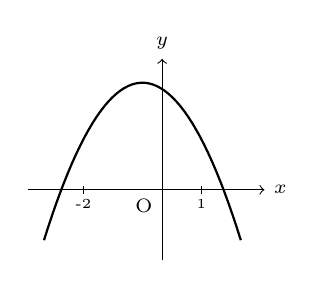
\begin{tikzpicture}[x=5mm,y=3.2mm]
\draw[->] (-3.4,0)--(2.6,0) node[right]{\scriptsize $x$};
\draw[->] (0,-2.8)--(0,5.2) node[above]{\scriptsize $y$};
\node[below left] at (0,0){\scriptsize O};
\draw[thick,domain=-3.0:2.0,samples=50] plot (\x,{-\x*\x-\x+4});
\foreach \t in {-2,1} {\draw (\t,0.15)--(\t,-0.15); \node[below] at (\t,0){\tiny \t};}
\end{tikzpicture}
\end{minipage}

\mon{46}{解の配置}
2次方程式 $x^2+2ax+a+2=0$ が次の条件をみたすような定数 $a$ の値の範囲をそれぞれ求めよ．
\begin{enumerate}
\item 異なる2つの正の解をもつ．
\item 正の解と負の解を1つずつもつ．
\item 異なる2つの解がともに $-1$ より大きい．
\end{enumerate}

\mon{47}{絶対不等式（Ⅰ）}
$x\geqq2$ をみたすすべての $x$ について，$2x+a\geqq0$ が成り立つような $a$ の値の範囲を求めよ．

\mon{48}{絶対不等式（Ⅱ）}
すべての $x$ に対して，$x^2+2ax+2a+8>0$ となるような $a$ の値の範囲を求めよ．

\mon{49}{文字係数の2次不等式}
$a$ を定数とする．$x$ の2次不等式 $x^2-(a+2)x+2a<0$ ……① について
\begin{enumerate}
\item ①を解け．
\item ①をみたす整数 $x$ がちょうど2個となるような $a$ の値の範囲を求めよ．
\end{enumerate}

\mon{50}{絶対値記号のついた2次方程式}
次の方程式を解け．
\[\text{(1)}\ \ x^2-3|x|-4=0\quad\cdots\cdots\text{①}\qquad\qquad\text{(2)}\ \ |x^2-x-6|=2x+4\quad\cdots\cdots\text{②}\]

\mon{51}{絶対値記号のついた2次不等式}
次の不等式を解け．
\[\text{(1)}\ \ x^2-|x|-6\leqq0\quad\cdots\cdots\text{①}\qquad\qquad\text{(2)}\ \ |x^2+4x+3|<2x+5\quad\cdots\cdots\text{②}\]

\shou{第4章}{図形の性質}
\mon{52}{三角形の重心，外心，内心，垂心}
$\triangle\mathrm{ABC}$ について，次の(1)〜(4)の点をそれぞれ何というか答えよ．また，外接円の中心，内接円の中心はそれぞれどれか答えよ．
\begin{enumerate}
\item 3辺の垂直二等分線の交点\qquad (2)\ 3つの内角の二等分線の交点
\item[(3)] 3本の中線の交点\qquad (4)\ 3つの頂点から対辺またはその延長に下ろした垂線の交点
\end{enumerate}

\mon{53}{角の2等分線の性質}
$\mathrm{AB}=6$，$\mathrm{BC}=5$，$\mathrm{CA}=4$ をみたす $\triangle\mathrm{ABC}$ について，
\begin{enumerate}
\item $\angle\mathrm{BAC}$ の2等分線と辺 BC の交点を D とするとき，$\mathrm{BD}:\mathrm{DC}$ を求めよ．
\item $\angle\mathrm{ABC}$ の2等分線と線分 AD の交点を I とおくとき，線分 BD の長さを求め，$\mathrm{AI}:\mathrm{ID}$ を求めよ．
\item 直線 BI と辺 CA の交点を E とするとき，$\mathrm{BI}:\mathrm{IE}$ を求めよ．
\end{enumerate}

\mon{54}{チェバの定理}
\begin{minipage}[t]{0.6\linewidth}
$\triangle\mathrm{ABC}$ において，辺 BC を $2:3$ に内分する点を D，辺 CA を $4:3$ に内分する点を E とする．また，AD と BE の交点を P とし，直線 CP と辺 AB との交点を F とする．このとき，$\mathrm{AF}:\mathrm{FB}$ を求めよ．
\end{minipage}\hfill
\begin{minipage}[t]{0.36\linewidth}
\vspace{-4pt}
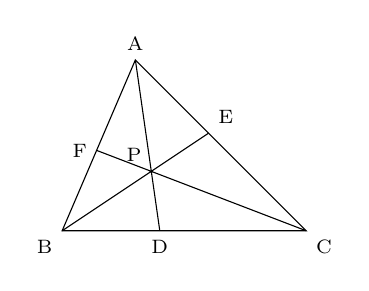
\begin{tikzpicture}[scale=0.62]
\coordinate (B) at (0,0); \coordinate (C) at (5,0); \coordinate (A) at (1.5,3.5);
\coordinate (D) at (2,0); \coordinate (E) at (3,2); \coordinate (F) at (0.706,1.647); \coordinate (P) at (1.826,1.217);
\draw (A)--(B)--(C)--cycle; \draw (A)--(D) (B)--(E) (C)--(F);
\node[above] at (A){\scriptsize A}; \node[below left] at (B){\scriptsize B}; \node[below right] at (C){\scriptsize C};
\node[below] at (D){\scriptsize D}; \node[above right] at (E){\scriptsize E}; \node[left] at (F){\scriptsize F}; \node[above left] at (P){\scriptsize P};
\end{tikzpicture}
\end{minipage}

\mon{55}{メネラウスの定理}
\begin{minipage}[t]{0.6\linewidth}
右図の $\triangle\mathrm{ABC}$ において，$\mathrm{AE}:\mathrm{EB}=1:2$，$\mathrm{BD}:\mathrm{DC}=2:1$ とし，AD と CE の交点を P とする．このとき，
\begin{enumerate}
\item $\mathrm{AP}:\mathrm{PD}$ を求めよ．
\item $\triangle\mathrm{PDC}:\triangle\mathrm{ABC}$ を求めよ．
\end{enumerate}
\end{minipage}\hfill
\begin{minipage}[t]{0.36\linewidth}
\vspace{-4pt}
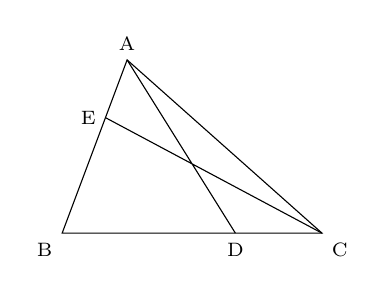
\begin{tikzpicture}[scale=0.55]
\coordinate (B) at (0,0); \coordinate (C) at (6,0); \coordinate (A) at (1.5,4);
\coordinate (D) at (4,0); \coordinate (E) at (1,2.667);
\draw (A)--(B)--(C)--cycle; \draw (A)--(D) (C)--(E);
\node[above] at (A){\scriptsize A}; \node[below left] at (B){\scriptsize B}; \node[below right] at (C){\scriptsize C};
\node[below] at (D){\scriptsize D}; \node[left] at (E){\scriptsize E};
\end{tikzpicture}
\end{minipage}

\mon{56}{円周角}
円 O に内接する四角形 ABCD の対角線 AC，BD の交点を P とする．$\angle\mathrm{ABD}=40^\circ$，$\angle\mathrm{BDC}=25^\circ$ のとき，次の問いに答えよ．
\begin{enumerate}
\item $\angle\mathrm{ACD}$，$\angle\mathrm{BAC}$ の大きさを求めよ．
\item $\angle\mathrm{AOD}$ の大きさを求めよ．
\item $\angle\mathrm{APB}$ の大きさを求めよ．
\item $\triangle\mathrm{ABP}\backsim\triangle\mathrm{DCP}$ であることを示せ．
\end{enumerate}

\mon{57}{接弦定理}
円周上に3点 A，B，C があり，点 A における円の接線上に，直線 AB に関して C と反対側に点 T をとる．$\angle\mathrm{TAB}=55^\circ$，$\angle\mathrm{ABC}=70^\circ$ のとき，次の問いに答えよ．
\begin{enumerate}
\item $\angle\mathrm{ACB}$ の大きさを求めよ．
\item $\angle\mathrm{BAC}$ の大きさを求めよ．
\item $\triangle\mathrm{ABC}$ はどのような三角形か．
\end{enumerate}

\mon{58}{方べきの定理}
\begin{minipage}[t]{0.6\linewidth}
右図のように，円外の点 O を通る2本の直線が円とそれぞれ A，B および C，D で交わっている．
\begin{enumerate}
\item $\triangle\mathrm{OAC}\backsim\triangle\mathrm{ODB}$ を示せ．
\item $\mathrm{OA}=3$，$\mathrm{OB}=8$，$\mathrm{OC}=4$ のとき，CD の長さを求めよ．
\end{enumerate}
\end{minipage}\hfill
\begin{minipage}[t]{0.37\linewidth}
\vspace{-4pt}
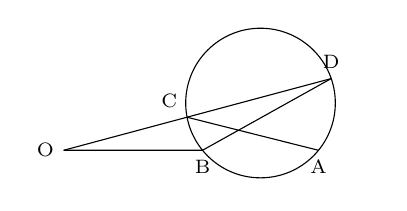
\begin{tikzpicture}[scale=0.5]
\coordinate (O) at (0,0); \coordinate (M) at (5,1.2);
\draw[name path=circ] (M) circle (1.9);
\path[name path=l1] (O)--(8,0); \path[name path=l2] (O)--($(O)!1!(15:8)$);
\draw[name intersections={of=circ and l1,by={B1,A1}}] (O)--(B1);
\draw[name intersections={of=circ and l2,by={D1,C1}}] (O)--(D1);
\draw (A1)--(C1) (B1)--(D1);
\node[left] at (O){\scriptsize O}; \node[below] at (A1){\scriptsize A}; \node[below] at (B1){\scriptsize B};
\node[above left] at (C1){\scriptsize C}; \node[above] at (D1){\scriptsize D};
\end{tikzpicture}
\end{minipage}

\mon{59}{2円の位置関係}
\begin{minipage}[t]{0.6\linewidth}
A を中心とする半径4の円 $C_1$ と B を中心とする半径9の円 $C_2$ が外接している．2円 $C_1$，$C_2$ の両方に接する直線と円 $C_1$，円 $C_2$ の接点をそれぞれ $\mathrm T_1$，$\mathrm T_2$ とする．
\begin{enumerate}
\item $\mathrm T_1\mathrm T_2$ の長さを求めよ．
\item 円 $C_1$ の半径を $a$，円 $C_2$ の半径を $b$（$a<b$）としたとき，$\mathrm T_1\mathrm T_2$ の長さを $a,\ b$ で表せ．
\end{enumerate}
\end{minipage}\hfill
\begin{minipage}[t]{0.37\linewidth}
\vspace{-4pt}
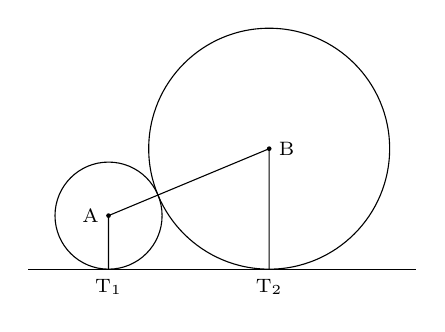
\begin{tikzpicture}[scale=0.17]
\coordinate (A) at (0,4); \coordinate (B) at (12,9);
\draw (A) circle (4); \draw (B) circle (9); \draw (-6,0)--(23,0);
\draw (A)--(B) (A)--(0,0) (B)--(12,0);
\fill (A) circle (5pt) (B) circle (5pt);
\node[left] at (A){\scriptsize A}; \node[right] at (B){\scriptsize B};
\node[below] at (0,0){\scriptsize $\mathrm T_1$}; \node[below] at (12,0){\scriptsize $\mathrm T_2$};
\end{tikzpicture}
\end{minipage}

\mon{60}{平面幾何（Ⅰ）}
$\triangle\mathrm{ABC}$ の辺 AB を $3:2$ に内分する点を D，辺 AC を $1:2$ に内分する点を E とし，直線 DE と直線 BC の交点を F とする．
\begin{enumerate}
\item $\mathrm{BF}:\mathrm{FC}$ を求めよ．
\item $\mathrm{AB}=10$ とする．4点 B，C，E，D が同一円周上にあるとき，AC の長さを求めよ．
\end{enumerate}

\mon{61}{平面幾何（Ⅱ）}
$\angle\mathrm A=90^\circ$，$\mathrm{AB}=6$，$\mathrm{AC}=8$ の直角三角形 ABC において，A から辺 BC に下ろした垂線を AH，辺 BC の中点を M とする．
\begin{enumerate}
\item AH，BH の長さを求めよ．
\item M は $\triangle\mathrm{ABC}$ の外心であることを示し，AM の長さを求めよ．
\item $\triangle\mathrm{AHM}$ の面積を求めよ．
\end{enumerate}

\mon{62}{四角形への応用（トレミーの定理）}
AC を直径とする円に四角形 ABCD が内接している．$\mathrm{AC}=5$，$\mathrm{AB}=\mathrm{AD}=3$ とする．
\begin{enumerate}
\item BC，CD の長さを求めよ．
\item トレミーの定理 $\mathrm{AB}\cdot\mathrm{CD}+\mathrm{BC}\cdot\mathrm{DA}=\mathrm{AC}\cdot\mathrm{BD}$ を用いて，BD の長さを求めよ．
\item (2)の結果を，BD と AC が垂直に交わることを用いて確かめよ．
\end{enumerate}

\mon{63}{内接球・外接球}
\begin{minipage}[t]{0.62\linewidth}
右図のように直円錐の底面と側面に球が内接している．直円錐の底面の半径を5，高さを12として，次の問いに答えよ．
\begin{enumerate}
\item 球の半径 $R$ を求めよ．
\item 直円錐の側面と球とが接する部分は円である．この円の半径 $r$ を求めよ．
\end{enumerate}
\end{minipage}\hfill
\begin{minipage}[t]{0.34\linewidth}
\vspace{-4pt}
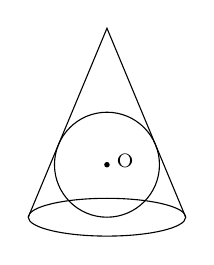
\begin{tikzpicture}[scale=0.2]
\draw (-5,0)--(0,12)--(5,0); \draw (0,0) ellipse (5 and 1.2);
\draw (0,3.333) circle (3.333); \fill (0,3.333) circle (5pt);
\node[right] at (0,3.6){\scriptsize O};
\end{tikzpicture}
\end{minipage}

\mon{64}{特殊な四面体（Ⅰ）}
$\mathrm{OA}=\mathrm{OB}=\mathrm{OC}=5$，$\mathrm{AB}=\mathrm{BC}=\mathrm{CA}=6$ の四面体 OABC がある．O から平面 ABC に下ろした垂線の足を H とする．
\begin{enumerate}
\item H は $\triangle\mathrm{ABC}$ の外心であることを示せ．
\item AH，OH の長さを求めよ．
\item 四面体 OABC の体積 $V$ を求めよ．
\end{enumerate}

\mon{65}{特殊な四面体（Ⅱ）}
1辺の長さが6の正四面体 ABCD について，次の問いに答えよ．
\begin{enumerate}
\item A から平面 BCD に下ろした垂線の長さ $h$ を求めよ．
\item 体積 $V$ を求めよ．
\item この正四面体に内接する球の半径 $r$ を求めよ．
\end{enumerate}


\shou{第5章}{図形と計量}
\mon{66}{鋭角の三角比}
次の図の直角三角形において，$\sin\theta$，$\cos\theta$，$\tan\theta$ の値を求めよ．\\[4pt]
\hspace*{2em}(1)\ 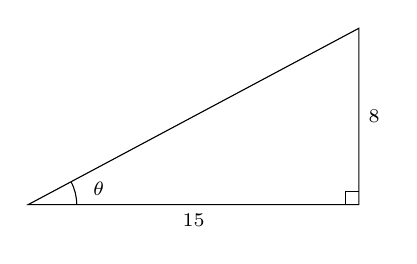
\begin{tikzpicture}[scale=0.28,baseline=0]
\draw (0,0)--(15,0)--(15,8)--cycle; \draw (14.4,0)--(14.4,0.6)--(15,0.6);
\draw (2.2,0) arc (0:28:2.2); \node at (3.2,0.7){\scriptsize $\theta$};
\node[below] at (7.5,0){\scriptsize 15}; \node[right] at (15,4){\scriptsize 8};
\end{tikzpicture}
\hspace{4em}(2)\ 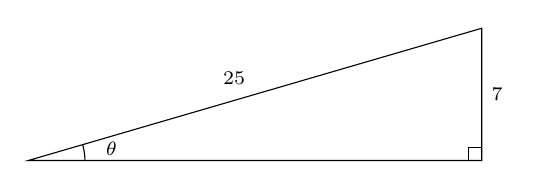
\begin{tikzpicture}[scale=0.24,baseline=0]
\draw (0,0)--(24,0)--(24,7)--cycle; \draw (23.3,0)--(23.3,0.7)--(24,0.7);
\draw (3,0) arc (0:16:3); \node at (4.4,0.6){\scriptsize $\theta$};
\node[above left] at (12,3.5){\scriptsize 25}; \node[right] at (24,3.5){\scriptsize 7};
\end{tikzpicture}

\mon{67}{有名角の三角比}
次の式の値を求めよ．
\[\text{(1)}\ \sin^260^\circ\qquad\text{(2)}\ 2\cos45^\circ-4\sin30^\circ\qquad\text{(3)}\ \tan30^\circ+\sin60^\circ\qquad\text{(4)}\ \cos60^\circ\cos30^\circ+\sin60^\circ\sin30^\circ\]

\mon{68}{鈍角の三角比}
次の三角比の値を，原点を中心とする半円（半径は自由に決めてよい）を利用して，それぞれ求めよ．
\[\text{(1)}\ \cos150^\circ\qquad\text{(2)}\ \sin135^\circ\qquad\text{(3)}\ \tan120^\circ\]

\mon{69}{補角・余角の三角比}
次の三角比を鋭角の三角比で表し，その値を求めよ．
\[\text{(1)}\ \sin150^\circ\qquad\text{(2)}\ \cos120^\circ\qquad\text{(3)}\ \tan135^\circ\]

\mon{70}{三角比の相互関係}
$0^\circ\leqq\theta\leqq180^\circ$ とするとき，次の問いに答えよ．
\begin{enumerate}
\item $\cos\theta=-\dfrac23$ のとき，$\sin\theta$，$\tan\theta$ の値を求めよ．
\item $\tan\theta=-2$ のとき，$\sin\theta$，$\cos\theta$ の値を求めよ．
\item $\sin\theta=\dfrac{5}{13}$ のとき，$\cos\theta$，$\tan\theta$ の値を求めよ．
\end{enumerate}

\mon{71}{三角比の計算（Ⅰ）}
次の式を簡単にせよ．
\[\text{(1)}\ \ (\sin\theta+\cos\theta)^2+(\sin\theta-\cos\theta)^2\qquad\qquad\text{(2)}\ \ \frac{\sin\theta}{1+\cos\theta}+\frac{1}{\tan\theta}\]

\mon{72}{三角比の計算（Ⅱ）}
$\sin\theta-\cos\theta=\dfrac12$ のとき，次の式の値を求めよ．
\[\text{(1)}\ \ \sin\theta\cos\theta\qquad\qquad\text{(2)}\ \ \sin^3\theta-\cos^3\theta\]

\mon{73}{三角方程式（Ⅰ）}
\begin{enumerate}
\item $0^\circ\leqq\theta\leqq180^\circ$ のとき，次の方程式を解け．\\
(i)\ $2\cos\theta=1$\qquad (ii)\ $\sqrt2\sin\theta-1=0$\qquad (iii)\ $\tan\theta+\sqrt3=0$
\item $0^\circ\leqq\theta\leqq90^\circ$ のとき，次の方程式を解け．\\
(i)\ $2\cos2\theta=-1$\qquad (ii)\ $2\sin2\theta=\sqrt3$\qquad (iii)\ $\sqrt3\tan2\theta=1$
\end{enumerate}

\mon{74}{三角不等式（Ⅰ）}
\begin{enumerate}
\item $0^\circ\leqq\theta\leqq180^\circ$ のとき，次の不等式を解け．\\
(i)\ $2\cos\theta\geqq1$\qquad (ii)\ $2\sin\theta-\sqrt3<0$\qquad (iii)\ $\tan\theta\geqq1$
\item $0^\circ\leqq\theta\leqq90^\circ$ のとき，次の不等式を解け．\\
(i)\ $2\cos2\theta>1$\qquad (ii)\ $2\sin2\theta-\sqrt3\geqq0$\qquad (iii)\ $\tan2\theta+\sqrt3<0$
\end{enumerate}

\mon{75}{三角方程式（Ⅱ）}
$2\cos^2x-3\sin x=0\ (0^\circ\leqq x\leqq180^\circ)$ について
\begin{enumerate}
\item $\sin x$ の値を求めよ．\qquad (2)\ $x$ の値を求めよ．
\end{enumerate}

\mon{76}{三角不等式（Ⅱ）}
$2\sin^2x+\cos x>2\ (0^\circ\leqq x\leqq180^\circ)$ について
\begin{enumerate}
\item $\cos x$ のとりうる値の範囲を求めよ．\qquad (2)\ $x$ の値の範囲を求めよ．
\end{enumerate}

\mon{77}{最大値・最小値}
$0^\circ\leqq x\leqq180^\circ$ のとき，$y=\cos^2x+\sin x$ ……① について，次の問いに答えよ．
\begin{enumerate}
\item $\sin x=t$ とおくとき，①を $t$ で表せ．
\item $t$ のとりうる値の範囲を求めよ．
\item ①の最大値，最小値とそのときの $x$ の値を求めよ．
\end{enumerate}

\mon{78}{正弦定理}
$\triangle\mathrm{ABC}$ について，次の問いに答えよ．
\begin{enumerate}
\item $\mathrm{CA}=3$，$\angle\mathrm A=75^\circ$，$\angle\mathrm C=60^\circ$ のとき，AB の長さを求めよ．
\item 外接円の半径 $R$ を求めよ．
\end{enumerate}

\mon{79}{余弦定理}
$\triangle\mathrm{ABC}$ において，$\mathrm{BC}=2$，$\mathrm{CA}=3$，$\angle\mathrm C=60^\circ$ が成りたっている．AB の長さを求めよ．

\mon{80}{正弦定理・余弦定理の使い分け}
$\triangle\mathrm{ABC}$ において，$\mathrm{AB}=5$，$\mathrm{CA}=7$，$\angle\mathrm B=60^\circ$ である．
\begin{enumerate}
\item BC の長さを求めよ．
\item $\sin C$ の値を求めよ．
\item 外接円の半径 $R$ を求めよ．
\end{enumerate}

\mon{81}{中線定理}
$\triangle\mathrm{ABC}$ において，辺 BC の中点を M とし，$\mathrm{AB}=c$，$\mathrm{BC}=2a$，$\mathrm{CA}=b$ とおくとき
\begin{enumerate}
\item $\cos C$ を $a,\ b,\ c$ で表せ．
\item $\triangle\mathrm{AMC}$ に着目して，$\mathrm{AM}^2$ を $a,\ b,\ c$ で表せ．
\item $\mathrm{AB}^2+\mathrm{AC}^2=2(\mathrm{AM}^2+\mathrm{BM}^2)$ が成りたつことを示せ．
\end{enumerate}

\mon{82}{三角形の重心}
$\mathrm{AB}=7$，$\mathrm{BC}=8$，$\mathrm{CA}=5$ の $\triangle\mathrm{ABC}$ において，辺 BC の中点を M，重心を G とする．
\begin{enumerate}
\item 中線 AM の長さを求めよ．
\item AG，GM の長さを求めよ．
\end{enumerate}

\mon{83}{三角形の形状決定}
次の等式が成りたつとき，$\triangle\mathrm{ABC}$ はどのような三角形か．
\[\text{(1)}\ \ \sin^2A=\sin^2B+\sin^2C\qquad\qquad\text{(2)}\ \ a\cos B=b\cos A\]

\mon{84}{三角形の成立条件}
3辺の長さが 4，5，$x$ である三角形について，
\begin{enumerate}
\item $x$ のとりうる値の範囲を求めよ．
\item この三角形が鋭角三角形となる $x$ の値の範囲を求めよ．
\item この三角形が鈍角三角形となる $x$ の値の範囲を求めよ．
\end{enumerate}

\mon{85}{三角形の面積}
次のような $\triangle\mathrm{ABC}$ の面積を求めよ．
\[\text{(1)}\ \ \mathrm{AB}=4,\ \mathrm{BC}=5,\ \angle\mathrm B=120^\circ\qquad\qquad\text{(2)}\ \ \mathrm{AB}=4,\ \mathrm{BC}=13,\ \mathrm{CA}=15\]

\mon{86}{角の2等分線の長さ}
$\angle\mathrm A=90^\circ$，$\mathrm{AB}=3$，$\mathrm{AC}=6$ の $\triangle\mathrm{ABC}$ において，$\angle\mathrm A$ の2等分線と辺 BC の交点を D とする．
\begin{enumerate}
\item BD の長さを求めよ．
\item $\triangle\mathrm{ABD}+\triangle\mathrm{ACD}=\triangle\mathrm{ABC}$ を用いて，AD の長さを求めよ．
\end{enumerate}

\mon{87}{内接円の半径（Ⅰ）}
$\mathrm{AB}=7$，$\mathrm{BC}=8$，$\mathrm{CA}=9$ をみたす $\triangle\mathrm{ABC}$ について
\begin{enumerate}
\item 面積を求めよ．\qquad (2)\ 内接円の半径 $r$ を求めよ．
\end{enumerate}

\mon{88}{内接円の半径（Ⅱ）}
$\angle\mathrm C=90^\circ$ の直角三角形 ABC において，$\mathrm{BC}=a$，$\mathrm{CA}=b$，$\mathrm{AB}=c$，内接円の半径を $r$ とする．
\begin{enumerate}
\item $a=5$，$b=12$ のとき，面積を利用して $r$ を求めよ．
\item 一般に $r=\dfrac{a+b-c}{2}$ が成りたつことを，内接円と各辺の接点を考えて示せ．
\end{enumerate}

\mon{89}{円に内接する四角形}
円に内接する四角形 ABCD において，$\mathrm{AB}=5$，$\mathrm{BC}=8$，$\angle\mathrm{ABC}=60^\circ$，$\mathrm{CD}=\mathrm{DA}$ である．
\begin{enumerate}
\item AC の長さを求めよ．\qquad (2)\ CD の長さを求めよ．
\item[(3)] 四角形 ABCD の面積を求めよ．\qquad (4)\ 外接円の半径 $R$ を求めよ．
\end{enumerate}


\shou{第6章}{順列・組合せ}
\mon{90}{場合の数（Ⅰ）}
10円玉4枚，100円玉2枚，500円玉2枚の一部，または全部を用いると，何種類の金額ができるか．

\mon{91}{場合の数（Ⅱ）}
\fbox{0}，\fbox{1}，\fbox{2} とかかれたカードが2枚ずつ計6枚ある．この6枚のうち，3枚を使って3桁の整数をつくるとき，次の問いに答えよ．ただし，同じ数字のカードは区別がつかないとする．
\begin{enumerate}
\item \fbox{0} を使わないものはいくつあるか．
\item \fbox{0} を使うものはいくつあるか．
\item 3桁の整数はいくつあるか．
\end{enumerate}

\mon{92}{場合の数（Ⅲ）}
0，1，2，3，4 の5種類の数字をくりかえし用いると，3桁の整数は何個できるか．

\mon{93}{約数の個数・総和}
108 の正の約数について
\begin{enumerate}
\item その個数を求めよ．\qquad (2)\ その総和を求めよ．
\end{enumerate}

\mon{94}{階乗，${}_n\mathrm P_r$，${}_n\mathrm C_r$ の計算}
\begin{enumerate}
\item 次の計算をせよ．\quad
(i)\ $7!-5!$\qquad (ii)\ $\dfrac{12!}{10!}$\qquad (iii)\ ${}_8\mathrm P_3$\qquad (iv)\ ${}_9\mathrm C_6$
\item 次の式が成りたつことを示せ．\quad
(i)\ ${}_n\mathrm P_r=r!\times{}_n\mathrm C_r$\qquad (ii)\ ${}_n\mathrm C_r={}_{n-1}\mathrm C_{r-1}+{}_{n-1}\mathrm C_r$
\end{enumerate}

\mon{95}{順列（Ⅰ）（場所指定）}
男子4人，女子3人の7人が横1列に並ぶとき，次のような並び方は何通りあるか．
\begin{enumerate}
\item 両端が男子である．
\item 女子3人が続けて並ぶ．
\item 女子どうしがとなりあわない．
\item 特定の3人 P，Q，R が，左からこの順に並ぶ（となりあわなくてもよい）．
\end{enumerate}

\mon{96}{倍数の規則}
0，1，2，3，4，5 の6個の数字から異なる3個を選んで並べ，3桁の整数をつくる．
\begin{enumerate}
\item 3桁の整数は全部でいくつあるか．
\item 5の倍数はいくつあるか．\qquad (3)\ 3の倍数はいくつあるか．
\item[(4)] 4の倍数はいくつあるか．\qquad (5)\ 15の倍数はいくつあるか．
\end{enumerate}

\mon{97}{順列（Ⅱ）（同じものを含む順列）}
committee の9個の文字を横一列に並べるとき，その並べ方は何通りあるか．

\mon{98}{順列（Ⅲ）（円順列）}
A，B を含む6人が円形のテーブルのまわりに等間隔に座る．
\begin{enumerate}
\item 座り方は全部で何通りあるか．
\item A と B がとなりあう座り方は何通りあるか．
\item A と B が向かいあう座り方は何通りあるか．
\end{enumerate}

\mon{99}{組合せ（Ⅰ）}
C，D 2人を含む12人から4人の委員を選ぶとき，
\begin{enumerate}
\item C，D をともに含む選び方は何通りあるか．
\item C は選ばれ，D は選ばれない選び方は何通りあるか．
\end{enumerate}

\mon{100}{組合せ（Ⅱ）}
正八角形について，次の問いに答えよ．
\begin{enumerate}
\item 対角線は何本あるか．
\item 8つの頂点から3点を選んでできる三角形は全部でいくつあるか．
\item (2)のうち，二等辺三角形はいくつあるか．
\item (2)のうち，正八角形と辺を共有しない三角形はいくつあるか．
\end{enumerate}

\mon{101}{組合せ（Ⅲ）}
1から10までの自然数から異なる4個を選ぶとき，
\begin{enumerate}
\item 選んだ数の最小値が3以上となる選び方は何通りあるか．
\item 最小値がちょうど3となる選び方は何通りあるか．
\item 最大値と最小値の差がちょうど5となる選び方は何通りあるか．
\end{enumerate}

\mon{102}{組分け（Ⅰ）}
6人の生徒を3つの部屋 A，B，C に入れる．
\begin{enumerate}
\item 空き部屋があってもよいとき，入れ方は何通りあるか．
\item ちょうど2つの部屋だけを使う入れ方は何通りあるか．
\item どの部屋にも少なくとも1人が入る入れ方は何通りあるか．
\end{enumerate}

\mon{103}{組分け（Ⅱ）}
6人を次のように分ける方法は，それぞれ何通りあるか．
\begin{enumerate}
\item 3人ずつ A，B の2組に分ける．\qquad (2)\ 3人ずつ2組に分ける．
\item[(3)] 2人ずつ A，B，C の3組に分ける．\qquad (4)\ 2人ずつ3組に分ける．
\item[(5)] 4人，1人，1人の3組に分ける．
\end{enumerate}

\mon{104}{道の数え方}
\begin{minipage}[t]{0.6\linewidth}
\begin{enumerate}
\item 右図①のような碁盤の目の道を A から B まで行くことを考える．\\
(i)\ 最短経路は何通りあるか．\\
(ii)\ (i)のうち，C を通るものは何通りあるか．
\item 右図②のように，区間 p，q（太線）が通れない道を A から B まで行くことを考える．最短経路は何通りあるか．
\end{enumerate}
\end{minipage}\hfill
\begin{minipage}[t]{0.38\linewidth}
\vspace{-4pt}
\begin{tikzpicture}[scale=0.42]
\draw (0,0) grid (4,4);
\node[below left] at (0,0){\scriptsize A}; \node[above right] at (4,4){\scriptsize B};
\fill (2,2) circle (3pt); \node[above left] at (2,2){\scriptsize C};
\node at (2,-1){\scriptsize ①};
\end{tikzpicture}\hspace{6pt}
\begin{tikzpicture}[scale=0.42]
\draw (0,0) grid (4,3);
\draw[line width=2pt] (1,1)--(2,1); \draw[line width=2pt] (3,1)--(3,2);
\node[below] at (1.5,1){\scriptsize p}; \node[right] at (3,1.5){\scriptsize q};
\node[below left] at (0,0){\scriptsize A}; \node[above right] at (4,3){\scriptsize B};
\node at (2,-1){\scriptsize ②};
\end{tikzpicture}
\end{minipage}

\mon{105}{重複組合せ}
区別のつかない球6個を A，B，C 3つの箱に入れる．
\begin{enumerate}
\item どの箱にも少なくとも1個の球が入る方法は何通りあるか．
\item 1個も入っていない箱があってもよいとすれば，何通りの方法があるか．
\end{enumerate}

\shou{第7章}{確率}
\mon{106}{同様な確からしさ（Ⅰ）}
大小2個のサイコロを同時に投げる．A さんは「出る目の和は2から12までの11通りだから，和が7になる確率は $\dfrac{1}{11}$ である」と考えた．
\begin{enumerate}
\item A さんの考えの誤りを指摘せよ．
\item 目の和が7になる確率を正しく求めよ．
\end{enumerate}

\mon{107}{同様な確からしさ（Ⅱ）}
1から12までの番号が1つずつ書かれた12枚のカードから同時に2枚を取り出す．
\begin{enumerate}
\item 2枚の番号の差がちょうど3である確率を求めよ．
\item 大きい方の番号が小さい方の番号の4倍以上である確率を求めよ．
\end{enumerate}

\mon{108}{同様な確からしさ（Ⅲ）}
1から6までの数字が1つずつ書かれたカードが6枚ある．この中から3枚を取り出して左から順に並べ，3桁の整数をつくる．
\begin{enumerate}
\item できる整数は全部で何個か．
\item できた整数が350以上である確率を求めよ．
\end{enumerate}

\mon{109}{排反事象}
赤球4個，白球3個，青球2個が入った袋から同時に2個を取り出すとき，2個が同じ色である確率を求めよ．

\mon{110}{余事象}
ある学級の生徒10人のうち4人が眼鏡をかけている．この10人から無作為に3人を選ぶとき，眼鏡をかけている人が少なくとも1人含まれる確率を求めよ．

\mon{111}{独立試行}
1枚の硬貨と1個のサイコロを同時に投げる試行を3回くりかえす．
\begin{enumerate}
\item 3回とも「硬貨が表で，サイコロの目が3の倍数」となる確率を求めよ．
\item 3回目にはじめて「硬貨が表で，サイコロの目が3の倍数」となる確率を求めよ．
\end{enumerate}

\mon{112}{反復試行}
命中率が $\dfrac23$ の選手がシュートを4回打つ．各シュートの結果は互いに影響しないものとする．
\begin{enumerate}
\item ちょうど3回命中する確率を求めよ．
\item 3回以上命中する確率を求めよ．
\end{enumerate}

\mon{113}{非復元抽出}
赤玉3個と白玉5個が入った箱から，A，B の2人がこの順に1個ずつ玉を取り出す．ただし，取り出した玉は箱にもどさない．
\begin{enumerate}
\item A が赤玉を取り出す確率を求めよ．
\item B が赤玉を取り出す確率を求めよ．
\end{enumerate}

\mon{114}{最大数・最小数の確率}
1から5までの数字が1つずつ書かれた5枚のカードから1枚引いて数字を記録し，カードをもとにもどす．これを3回行い，記録した数のうち最小のものを $Y$ とする．
\begin{enumerate}
\item $Y\geqq3$ となる確率を求めよ．
\item $Y=3$ となる確率を求めよ．
\end{enumerate}

\mon{115}{点の移動}
座標平面上の点 P は最初原点にある．サイコロを1回投げるごとに，2以下の目が出たら $x$ 軸の正の方向に1，3以上の目が出たら $y$ 軸の正の方向に1だけ動く．サイコロを6回投げる．
\begin{enumerate}
\item 2以下の目が $k$ 回出たときの P の座標を $k$ で表せ．
\item P が点 $(2,\ 4)$ にある確率を求めよ．
\end{enumerate}

\mon{116}{カードの確率}
1，2，3，4 の数字が書かれたカードが，赤と白の2色について1枚ずつ，計8枚ある．この8枚から同時に3枚を取り出す．
\begin{enumerate}
\item 取り出し方の総数を求めよ．
\item 3枚の中に同じ数字のカードが含まれる確率を求めよ．
\item 3枚とも同じ色である確率を求めよ．
\end{enumerate}

\mon{117}{一般の加法定理}
1から30までの番号が書かれたカードから1枚を引く．事象 $A$，$B$ を
\[A:\ \text{番号が4の倍数}\qquad B:\ \text{番号が6の倍数}\]
と定める．
\begin{enumerate}
\item $P(A)$，$P(B)$，$P(A\cap B)$，$P(A\cup B)$ を求めよ．
\item $A$，$B$ のどちらか一方だけが起こる確率を求めよ．
\end{enumerate}

\mon{118}{道の確率}
\begin{minipage}[t]{0.62\linewidth}
右図のような道があり，P から Q まで最短経路で進む．
\begin{enumerate}
\item 最短経路のうちの1つを選ぶことが同様に確からしいとして，R を通る確率を求めよ．
\item 各交差点で，上へ行くか右へ行くかを確率 $\dfrac12$ ずつで選ぶとする（一方にしか進めないときはその方向に進む）．R を通る確率を求めよ．
\end{enumerate}
\end{minipage}\hfill
\begin{minipage}[t]{0.34\linewidth}
\vspace{-4pt}
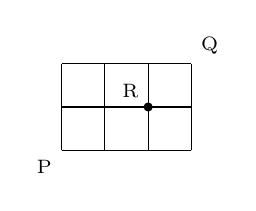
\begin{tikzpicture}[scale=0.55]
\draw (0,0) grid (3,2);
\node[below left] at (0,0){\scriptsize P}; \node[above right] at (3,2){\scriptsize Q};
\fill (2,1) circle (3pt); \node[above left] at (2,1){\scriptsize R};
\end{tikzpicture}
\end{minipage}

\mon{119}{確率の最大値}
赤玉3個と白玉 $n$ 個（$n\geqq1$）が入った袋から同時に3個を取り出すとき，赤玉1個，白玉2個である確率を $p_n$ とする．
\begin{enumerate}
\item $p_n$ を $n$ で表せ．
\item $p_n$ を最大にする $n$ を求めよ．
\end{enumerate}

\mon{120}{条件付確率（Ⅰ）}
ある高校の2年生200人について，部活動への所属と通学方法を調べたところ，次の表のようになった．
\begin{center}
\renewcommand{\arraystretch}{1.2}
\begin{tabular}{c|cc|c}
 & 運動部 & 運動部以外 & 計\\ \hline
自転車通学 & 48 & 32 & 80\\
自転車以外 & 52 & 68 & 120\\ \hline
計 & 100 & 100 & 200
\end{tabular}
\end{center}
この200人から1人を選ぶとき，
\begin{enumerate}
\item 選ばれた生徒が運動部で自転車通学である確率を求めよ．
\item 選ばれた生徒が自転車通学であるとわかったとき，その生徒が運動部である条件付確率を求めよ．
\end{enumerate}

\mon{121}{条件付確率（Ⅱ）}
ある製品は工場 X で全体の 60\,\%，工場 Y で 40\,\% が作られている．X の製品の 2\,\%，Y の製品の 5\,\% が不良品である．全製品の中から1個を選ぶ．
\begin{enumerate}
\item 選んだ製品が不良品である確率を求めよ．
\item 選んだ製品が不良品であったとき，それが工場 Y の製品である確率を求めよ．
\end{enumerate}

\mon{122}{期待値（Ⅰ）}
赤玉4個と白玉6個が入った袋から同時に3個を取り出すとき，取り出した赤玉の個数の期待値を求めよ．

\mon{123}{期待値（Ⅱ）}
1から6までの数字が書かれた6枚のカードから同時に2枚を取り出し，小さい方の数字を $X$ とする．
\begin{enumerate}
\item $X=2$ となる確率を求めよ．
\item $X$ の期待値を求めよ．
\end{enumerate}

\shou{第8章}{データの分析}
\mon{124}{度数分布表とヒストグラム}
次のデータは，ある部活動の部員20人の体力テストの得点である．
\[52,\ 67,\ 71,\ 45,\ 88,\ 63,\ 59,\ 74,\ 81,\ 66,\ 38,\ 70,\ 57,\ 92,\ 64,\ 76,\ 49,\ 68,\ 73,\ 55\]
\begin{enumerate}
\item 30点以上40点未満から始めて，階級の幅を10点とする度数分布表をつくれ．
\item (1)の度数分布表をもとに，ヒストグラムをかけ．
\end{enumerate}

\mon{125}{データの代表値（平均値・メジアン・モード）}
10人の生徒が1か月に読んだ本の冊数を調べたところ，次のようになった．
\[3,\ 7,\ 5,\ 8,\ 5,\ 6,\ 9,\ 5,\ 4,\ 8\]
このデータの平均値，中央値（メジアン），最頻値（モード）を求めよ．

\mon{126}{四分位数}
次のデータは，11人のハンドボール投げの記録（単位 m）である．
\[12,\ 25,\ 18,\ 30,\ 22,\ 15,\ 27,\ 20,\ 33,\ 16,\ 24\]
第1四分位数 $Q_1$，第2四分位数 $Q_2$，第3四分位数 $Q_3$，および四分位範囲を求めよ．

\mon{127}{ヒストグラムと四分位数}
40人の通学時間（分）を調べ，次の度数分布表にまとめた．
\begin{center}
\renewcommand{\arraystretch}{1.15}
\begin{tabular}{c|ccccc|c}
階級（分） & 0〜10 & 10〜20 & 20〜30 & 30〜40 & 40〜50 & 計\\ \hline
度数（人） & 4 & 8 & 12 & 10 & 6 & 40
\end{tabular}
\end{center}
（階級は「〜以上〜未満」を表す．）第1四分位数，中央値，第3四分位数は，それぞれどの階級に含まれるか．

\mon{128}{箱ひげ図}
類題126のデータの箱ひげ図をかけ．

\mon{129}{ヒストグラムと箱ひげ図}
類題127のデータについて，最小値は2分，最大値は48分であった．このデータの箱ひげ図として考えられるものを，次の①〜③から1つ選べ．ただし，それぞれ（最小値，$Q_1$，中央値，$Q_3$，最大値）を表している．
\[\text{①}\ (2,\ 8,\ 25,\ 33,\ 48)\qquad\text{②}\ (2,\ 15,\ 27,\ 35,\ 48)\qquad\text{③}\ (2,\ 14,\ 31,\ 38,\ 48)\]

\mon{130}{箱ひげ図の比較}
A 組，B 組（ともに40人）の数学のテストの得点について，次のことがわかっている．
\begin{center}
\renewcommand{\arraystretch}{1.15}
\begin{tabular}{c|ccccc}
 & 最小値 & $Q_1$ & 中央値 & $Q_3$ & 最大値\\ \hline
A 組 & 22 & 45 & 58 & 70 & 95\\
B 組 & 30 & 52 & 60 & 66 & 88
\end{tabular}
\end{center}
次の(1)〜(4)のうち，このデータから必ず正しいといえるものをすべて選べ．
\begin{enumerate}
\item 範囲は A 組の方が大きい．
\item 四分位範囲は B 組の方が小さい．
\item 60点以上の生徒は B 組に20人以上いる．
\item 平均点は B 組の方が高い．
\end{enumerate}

\mon{131}{外れ値}
次の10個のデータについて，「$Q_1-1.5\times(\text{四分位範囲})$ 以下，または $Q_3+1.5\times(\text{四分位範囲})$ 以上の値」を外れ値とする．外れ値があればすべて答えよ．
\[5,\ 8,\ 9,\ 10,\ 11,\ 12,\ 13,\ 14,\ 15,\ 26\]

\mon{132}{分散・標準偏差}
5個のデータ $4,\ 8,\ 6,\ 5,\ 7$ の分散と標準偏差を求めよ．

\mon{133}{計算の工夫}
5個のデータ $1003,\ 1006,\ 1001,\ 1008,\ 1007$ の平均値と分散を，$y=x-1005$ と変換して求めよ．

\mon{134}{もう1つの分散の求め方}
5個のデータ $2,\ 4,\ 4,\ 5,\ 10$ の分散を，
\begin{enumerate}
\item 偏差の2乗の平均として求めよ．
\item $(\text{2乗の平均})-(\text{平均})^2$ として求め，(1)と一致することを確かめよ．
\end{enumerate}

\mon{135}{代表値の変化（データの合算）}
グループ A（6人）の得点の平均値は50，分散は16，グループ B（4人）の得点の平均値は60，分散は36である．2つのグループを合わせた10人の得点の平均値と分散を求めよ．

\mon{136}{代表値の変化（データの追加）}
9個のデータの平均値が10，分散が4である．このデータに値20を1個追加した10個のデータの平均値と分散を求めよ．

\mon{137}{代表値の変化（変量変換）}
変量 $x$ のデータの平均値が20，分散が9である．
\begin{enumerate}
\item $y=2x-5$ で定まる変量 $y$ の平均値，分散，標準偏差を求めよ．
\item $z=\dfrac{x-20}{3}$ で定まる変量 $z$ の平均値と標準偏差を求めよ．
\end{enumerate}

\mon{138}{偏差値}
得点 $x$ の偏差値を $50+10\times\dfrac{x-\overline x}{s}$（$\overline x$ は平均値，$s$ は標準偏差）で定める．あるテストの平均点が58点，標準偏差が12点であった．
\begin{enumerate}
\item 76点の生徒の偏差値を求めよ．
\item 偏差値が40である生徒の得点を求めよ．
\end{enumerate}

\mon{139}{散布図と相関}
次の①〜③の散布図について，2つの変量の間にある相関を「正の相関」「負の相関」「相関はほとんどない」のいずれかで答えよ．\\[4pt]
\begin{center}
\begin{tikzpicture}[scale=0.5]
\draw[->] (0,0)--(5,0); \draw[->] (0,0)--(0,5);
\foreach \p in {(0.5,4.4),(1,3.9),(1.4,4.1),(1.8,3.2),(2.3,3.0),(2.6,2.4),(3.1,2.2),(3.4,1.5),(3.9,1.4),(4.3,0.8)} \fill \p circle (2.5pt);
\node at (2.5,-0.8){\scriptsize ①};
\end{tikzpicture}\hspace{2em}
\begin{tikzpicture}[scale=0.5]
\draw[->] (0,0)--(5,0); \draw[->] (0,0)--(0,5);
\foreach \p in {(0.6,2.5),(1,4.2),(1.3,1.1),(1.9,3.3),(2.2,0.7),(2.6,2.8),(3,4.4),(3.5,1.6),(3.9,3.6),(4.3,2.1)} \fill \p circle (2.5pt);
\node at (2.5,-0.8){\scriptsize ②};
\end{tikzpicture}\hspace{2em}
\begin{tikzpicture}[scale=0.5]
\draw[->] (0,0)--(5,0); \draw[->] (0,0)--(0,5);
\foreach \p in {(0.5,0.9),(0.9,1.6),(1.4,1.2),(1.8,2.2),(2.2,2.0),(2.7,2.9),(3.1,2.6),(3.5,3.6),(3.9,3.4),(4.3,4.3)} \fill \p circle (2.5pt);
\node at (2.5,-0.8){\scriptsize ③};
\end{tikzpicture}
\end{center}

\mon{140}{散布図（読みとり）}
\begin{minipage}[t]{0.55\linewidth}
右の散布図は，10人の生徒の数学と英語の得点を表したものである．
\begin{enumerate}
\item 数学の得点が英語の得点より高い生徒は何人か．
\item 数学と英語がともに70点以上の生徒は何人か．
\end{enumerate}
\end{minipage}\hfill
\begin{minipage}[t]{0.42\linewidth}
\vspace{-4pt}
\begin{tikzpicture}[x=0.65mm,y=0.65mm]
\draw[->] (30,30)--(100,30) node[right]{\scriptsize 数学};
\draw[->] (30,30)--(30,100) node[above]{\scriptsize 英語};
\foreach \t in {40,50,...,90} {\draw[gray!40] (\t,30)--(\t,95); \draw[gray!40] (30,\t)--(95,\t);
  \node[below] at (\t,30){\tiny \t}; \node[left] at (30,\t){\tiny \t};}
\draw[dashed] (30,30)--(95,95);
\foreach \p in {(40,55),(50,45),(55,60),(60,65),(65,55),(70,75),(75,70),(80,85),(85,75),(90,80)} \fill \p circle (1.2pt);
\end{tikzpicture}
\end{minipage}

\mon{141}{共分散・相関係数}
2つの変量 $x,\ y$ のデータが次のように与えられている．
\begin{center}
\begin{tabular}{c|ccccc}
$x$ & 1 & 3 & 5 & 7 & 9\\ \hline
$y$ & 1 & 2 & 3 & 5 & 4
\end{tabular}
\end{center}
$x$ と $y$ の共分散 $s_{xy}$，および相関係数 $r$ を求めよ．

\mon{142}{仮説検定の考え方}
あるコインを10回投げたところ，表が9回出た．このコインは表が出やすいと判断してよいか．「表と裏の出やすさは同じ」という仮説のもとで，表が9回以上出る確率を求め，基準となる確率を5\,\% として判断せよ．

\shou{第9章}{整数の性質}
\mon{143}{最大公約数・最小公倍数}
最大公約数が12，最小公倍数が360である2つの自然数 $a,\ b$（$a<b$）の組をすべて求めよ．

\mon{144}{倍数の証明}
すべての整数 $n$ について，$n^3+5n$ は6の倍数であることを示せ．

\mon{145}{整数の余りによる分類}
\begin{enumerate}
\item 整数の2乗を4で割った余りは0または1であることを示せ．
\item $a^2+b^2=4c+3$ をみたす整数 $a,\ b,\ c$ は存在しないことを示せ．
\end{enumerate}

\mon{146}{ユークリッドの互除法}
互除法を用いて，1547 と 1183 の最大公約数を求めよ．

\mon{147}{不定方程式 $ax+by=c$ の解}
\begin{enumerate}
\item $13x+8y=1$ をみたす整数 $x,\ y$ の組を1つ求めよ．
\item $13x+8y=1$ をみたす整数 $x,\ y$ の組をすべて求めよ．
\item $13x+8y=5$ をみたす整数 $x,\ y$ の組をすべて求めよ．
\end{enumerate}

\mon{148}{2進法}
\begin{enumerate}
\item 10進法で表された数 45 を2進法で表せ．
\item 2進法で表された数 $1101011_{(2)}$ を10進法で表せ．
\end{enumerate}

\mon{149}{2進法の計算}
次の計算をし，結果を2進法で答えよ．
\[\text{(1)}\ \ 1011_{(2)}+111_{(2)}\qquad\qquad\text{(2)}\ \ 1011_{(2)}\times101_{(2)}\]

\mon{150}{整数問題（Ⅰ）}
$xy-2x-3y=0$ をみたす自然数 $x,\ y$ の組をすべて求めよ．

\mon{151}{整数問題（Ⅱ）}
$\dfrac1x+\dfrac1y+\dfrac1z=1$ をみたす自然数 $x,\ y,\ z$（$x\leqq y\leqq z$）の組をすべて求めよ．

\mon{152}{整数問題（Ⅲ）}
$x^2-y^2=24$ をみたす自然数 $x,\ y$ の組をすべて求めよ．

\mon{153}{ガウス記号（Ⅰ）}
実数 $x$ に対して，$x$ を超えない最大の整数を $[x]$ で表す．
\begin{enumerate}
\item $[2x-1]=3$ をみたす $x$ の値の範囲を求めよ．
\item $[x]^2-[x]-2=0$ をみたす $x$ の値の範囲を求めよ．
\end{enumerate}

\mon{154}{ガウス記号（Ⅱ）}
\begin{enumerate}
\item $50!$ を素因数分解したときの素因数2の個数を求めよ．
\item $50!$ を計算すると，末尾に0は連続していくつ並ぶか．
\end{enumerate}

\clearpage
{\sffamily\bfseries\Huge 解答\par}\vspace{4pt}\hrule height 1.5pt
\shouans{第1章}{数と式}


\ans{1}{指数の計算}
\begin{kai}
(1)\ $2^{4+3}=2^7=128$\qquad (2)\ $3^{2\times3}=3^6=729$\qquad (3)\ $x^{3+1}y^{1+4}=x^4y^5$\\[2pt]
(4)\ $3\cdot2\cdot5\,x^{2+1}y^{1+3+1}z^{1+2}=30x^3y^5z^3$\\[2pt]
(5)\ $9x^4y^2\times(-8x^3y^6)=-72x^7y^8$
\end{kai}

\ans{2}{整式の加減}
\begin{kai}
$A+B=(2x^2+x^2)+(-3x+5x)+(1-4)=3x^2+2x-3$\\
$A-B=(2x^2-x^2)+(-3x-5x)+(1+4)=x^2-8x+5$\qquad \point{引くときは $B$ の全部の項の符号が変わる}
\end{kai}

\ans{3}{式の展開}
\begin{kai}
(1)\ \point{$x-z=u$ とおく}\quad $(u+y)(u-y)=u^2-y^2=x^2-2xz+z^2-y^2$\\
\hspace*{1.5em}$=x^2-y^2+z^2-2xz$\\[2pt]
(2)\ $x^2-x=t$ とおくと $(t+1)(2t-3)=2t^2-t-3=2(x^2-x)^2-(x^2-x)-3$\\
\hspace*{1.5em}$=2x^4-4x^3+2x^2-x^2+x-3=2x^4-4x^3+x^2+x-3$\\[2pt]
(3)\ \point{$x^2+x$ が共通に出る組をつくる}\quad $\{(x-1)(x+2)\}\{(x-3)(x+4)\}=(x^2+x-2)(x^2+x-12)$\\
\hspace*{1.5em}$x^2+x=t$ とおくと $(t-2)(t-12)=t^2-14t+24$\\
\hspace*{1.5em}$=x^4+2x^3+x^2-14x^2-14x+24=x^4+2x^3-13x^2-14x+24$\\[2pt]
(4)\ $(x^2-4)(x^2+4)=x^4-16$\\[2pt]
(5)\ \point{$(a+b+c)(a^2+b^2+c^2-ab-bc-ca)=a^3+b^3+c^3-3abc$ の $b,\ c$ を $-b,\ -c$ にしたもの}\\
\hspace*{1.5em}$a^3+(-b)^3+(-c)^3-3a(-b)(-c)=a^3-b^3-c^3-3abc$
\end{kai}

\ans{4}{因数分解}
\begin{kai}
(1)\ $x^2(3x+2)-4(3x+2)=(x^2-4)(3x+2)=(x+2)(x-2)(3x+2)$\\[2pt]
(2)\ \point{$x$ について整理}\quad $(y-1)x-(y-1)=(x-1)(y-1)$\\[2pt]
(3)\ $ab(2a^2+ab-3b^2)=ab(2a+3b)(a-b)$\\[2pt]
(4)\ $(x^2-1)(x^2-9)=(x+1)(x-1)(x+3)(x-3)$\\[2pt]
(5)\ $x^2+x=t$ とおくと $(t-5)(t-3)-3=t^2-8t+12=(t-2)(t-6)$\\
\hspace*{1.5em}$=(x^2+x-2)(x^2+x-6)=(x+2)(x-1)(x+3)(x-2)$\\[2pt]
(6)\ \point{$z$ について整理}\quad $(xy-x-y+1)z-(xy-x-y+1)=(xy-x-y+1)(z-1)$\\
\hspace*{1.5em}$=(x-1)(y-1)(z-1)$
\end{kai}

\ans{5}{対称式}
\begin{kai}
(1)\ (i)\ $(x+y)^2-2xy=9-2=7$\qquad (ii)\ $(x+y)^3-3xy(x+y)=27-9=18$\\
\hspace*{1.5em}(iii)\ $(x^2+y^2)^2-2(xy)^2=49-2=47$\\[2pt]
(2)\ (i)\ $\left(x+\dfrac1x\right)^2-2=9-2=7$\qquad (ii)\ $\left(x+\dfrac1x\right)^3-3\left(x+\dfrac1x\right)=27-9=18$\\[2pt]
(3)\ (i)\ $(x+y+z)^2-2(xy+yz+zx)=4+2=6$\\
\hspace*{1.5em}(ii)\ $(xy+yz+zx)^2-2xyz(x+y+z)=1-2\cdot(-2)\cdot2=9$
\end{kai}

\ans{6}{実数（有理数・無理数）}
\begin{kai}
(1)\ (i)\ $x=\rpt7$ とおくと $10x-x=7$，$x=\dfrac79$\qquad
(ii)\ $100y-y=45$，$y=\dfrac{45}{99}=\dfrac5{11}$\\[2pt]
\hspace*{1.5em}(iii)\ $1000z-z=216$，$z=\dfrac{216}{999}=\dfrac{8}{37}$\\[2pt]
(2)\ (i)\ $3\div7=0.428571428571\cdots$ より\quad $\dfrac37=0.\dot42857\dot1$\\[2pt]
\hspace*{1.5em}(ii)\ \point{6個の数字のくり返し}\quad $2000=6\times333+2$ より，小数第2位の数字と同じで\quad $2$
\end{kai}

\ans{7}{無理数の計算（有理化）}
\begin{kai}
(1)\ $\dfrac{\sqrt7-2}{(\sqrt7+2)(\sqrt7-2)}=\dfrac{\sqrt7-2}{7-4}=\dfrac{\sqrt7-2}{3}$\\[4pt]
(2)\ \point{$(2+\sqrt2)^2-(\sqrt6)^2$ で $\sqrt{\ }$ が1つ減る}\\
\hspace*{1.5em}$\dfrac{2+\sqrt2-\sqrt6}{(2+\sqrt2)^2-6}=\dfrac{2+\sqrt2-\sqrt6}{4\sqrt2}
=\dfrac{(2+\sqrt2-\sqrt6)\sqrt2}{8}=\dfrac{2\sqrt2+2-2\sqrt3}{8}=\dfrac{1+\sqrt2-\sqrt3}{4}$
\end{kai}

\ans{8}{無理数の計算（数値代入）}
\begin{kai}
(1)\ \point{$\sqrt5$ を単独にして2乗}\quad $2x-1=\sqrt5$ より $4x^2-4x+1=5$，$x^2-x=1$\\[2pt]
(2)\ (1)より $x^2=x+1$．$x^3=x\cdot x^2=x^2+x=2x+1$．\\
\hspace*{1.5em}$2x^3-3x^2-x+4=2(2x+1)-3(x+1)-x+4=3$
\end{kai}

\ans{9}{無理数の大小比較}
\begin{kai}
(1)\ $16<19<25$ より $\sqrt{16}<\sqrt{19}<\sqrt{25}$．\quad よって $4<\sqrt{19}<5$\\
\hspace*{1.5em}\point{示すべき式を先に書かない．根拠 → 結論の順に書く}\\[2pt]
(2)\ $\dfrac{1}{3-\sqrt7}=\dfrac{3+\sqrt7}{9-7}=\dfrac{3+\sqrt7}{2}$，\quad
$\dfrac{2}{\sqrt{11}-\sqrt7}=\dfrac{2(\sqrt{11}+\sqrt7)}{11-7}=\dfrac{\sqrt{11}+\sqrt7}{2}$\\[2pt]
\hspace*{1.5em}$9<11$ より $3<\sqrt{11}$．両辺に $\sqrt7$ を加えて2で割ると\quad
$\dfrac{1}{3-\sqrt7}<\dfrac{2}{\sqrt{11}-\sqrt7}$
\end{kai}

\ans{10}{整数部分・小数部分}
\begin{kai}
(1)\ $4<7<9$ より $2<\sqrt7<3$．\quad $a=2$，$b=\sqrt7-2$\\[2pt]
(2)\ \point{$b+2=\sqrt7$ を利用}\quad $b(b+4)=(b+2)^2-4=7-4=3$\\[2pt]
(3)\ $\dfrac1b=\dfrac1{\sqrt7-2}=\dfrac{\sqrt7+2}{3}$．$4<\sqrt7+2<5$ より $\dfrac43<\dfrac1b<\dfrac53$．\quad 整数部分は\quad 1
\end{kai}

\ans{11}{絶対値記号}
\begin{kai}
(1)\ $\sqrt3-2<0$，$1-\sqrt3<0$ だから\quad $-(\sqrt3-2)-(1-\sqrt3)=1$\\[2pt]
(2)\ (i)\ $x<-2$ のとき $P=-(x+2)-(x-3)=-2x+1$\\
\hspace*{1.5em}(ii)\ $-2\leqq x\leqq3$ のとき $P=(x+2)-(x-3)=5$\\
\hspace*{1.5em}(iii)\ $3<x$ のとき $P=(x+2)+(x-3)=2x-1$
\end{kai}

\ans{12}{文字式の平方根}
\begin{kai}
\point{$\sqrt{A^2}=|A|$}\quad 与式 $=\sqrt{(x-2)^2}+\sqrt{(x+3)^2}=|x-2|+|x+3|$\\[2pt]
$x<-3$ のとき\quad $-(x-2)-(x+3)=-2x-1$\\
$-3\leqq x\leqq2$ のとき\quad $-(x-2)+(x+3)=5$\\
$2<x$ のとき\quad $(x-2)+(x+3)=2x+1$
\end{kai}

\ans{13}{2重根号}
\begin{kai}
(1)\ たして7，かけて10 は 5 と 2．\quad $(\sqrt5+\sqrt2)+(\sqrt5-\sqrt2)=2\sqrt5$\\[2pt]
(2)\ $4\sqrt6=2\sqrt{24}$．たして11，かけて24 は 8 と 3．\\
\hspace*{1.5em}$\sqrt{11\mp2\sqrt{24}}=\sqrt8\mp\sqrt3=2\sqrt2\mp\sqrt3$（複号同順）．\quad
与式 $=(2\sqrt2-\sqrt3)-(2\sqrt2+\sqrt3)=-2\sqrt3$\\[2pt]
(3)\ \point{内側の $\sqrt{\ }$ の前に2をつくる}\quad
$\sqrt{4\pm\sqrt{15}}=\sqrt{\dfrac{8\pm2\sqrt{15}}{2}}=\dfrac{\sqrt5\pm\sqrt3}{\sqrt2}$（複号同順）\\[2pt]
\hspace*{1.5em}与式 $=\dfrac{(\sqrt5+\sqrt3)-(\sqrt5-\sqrt3)}{\sqrt2}=\dfrac{2\sqrt3}{\sqrt2}=\sqrt6$
\end{kai}

\ans{14}{文字係数の方程式}
\begin{kai}
$(a-1)x=b-2$ と変形する．\point{$a-1$ で割れるかどうかで場合分け}\\
(i)\ $a\neq1$ のとき\quad $x=\dfrac{b-2}{a-1}$\\
(ii)\ $a=1$ のとき，方程式は $0\cdot x=b-2$．\\
\hspace*{1.5em}$b\neq2$ のとき，これをみたす $x$ は存在しない．\quad $b=2$ のとき，すべての $x$ がみたす．\\[2pt]
以上より\quad
$\begin{cases}a\neq1\ \text{のとき，}\ x=\dfrac{b-2}{a-1}\\ a=1,\ b\neq2\ \text{のとき，解なし}\\ a=1,\ b=2\ \text{のとき，すべての実数}\end{cases}$
\end{kai}

\ans{15}{1次不等式}
\begin{kai}
(1)\ $3x-5x>-4-2$，$-2x>-6$．\point{負の数で割ると向きが逆}\quad $x<3$\\[2pt]
(2)\ 両辺を12倍して $8x-6\geqq9x-4$，$-x\geqq2$．\quad $x\leqq-2$
\end{kai}

\ans{16}{連立不等式}
\begin{kai}
①は $2x>6$ より $x>3$．\quad ②は $3x\leqq15$ より $x\leqq5$．\\
数直線で重なった部分をとって\quad $3<x\leqq5$
\end{kai}

\ans{17}{文字係数の1次不等式}
\begin{kai}
(i)\ $a>0$ のとき\quad $x<\dfrac ba$\qquad
(ii)\ $a<0$ のとき\quad $x>\dfrac ba$\quad\point{負の数で割ると向きが逆}\\[2pt]
(iii)\ $a=0$ のとき，不等式は $0\cdot x<b$．左辺はつねに0なので，\\
\hspace*{1.5em}$b>0$ のとき，すべての実数．\quad $b\leqq0$ のとき，解なし．
\end{kai}

\ans{18}{絶対値記号のついた1次方程式}
\begin{kai}
(1)\ $x+2=\pm3$ より\quad $x=1,\ -5$\\[2pt]
(2)\ \point{絶対値の中身が0になる $x=0,\ 2$ で場合分け}\\
\hspace*{1.5em}(i)\ $x<0$ のとき\quad $-x-(x-2)=4$，$x=-1$．これは $x<0$ をみたす．\\
\hspace*{1.5em}(ii)\ $0\leqq x\leqq2$ のとき\quad $x-(x-2)=4$，$0\cdot x=2$ となり，解なし．\\
\hspace*{1.5em}(iii)\ $2<x$ のとき\quad $x+(x-2)=4$，$x=3$．これは $2<x$ をみたす．\\
\hspace*{1.5em}よって\quad $x=-1,\ 3$
\end{kai}

\ans{19}{絶対値記号のついた1次不等式}
\begin{kai}
(1)\ $-3<x+1<3$ より\quad $-4<x<2$\\[2pt]
(2)\ (i)\ $x<0$ のとき\quad $-x-(x-2)<4$，$x>-1$．よって $-1<x<0$\\
\hspace*{1.5em}(ii)\ $0\leqq x\leqq2$ のとき\quad $x-(x-2)<4$，$0\cdot x<2$ はつねに成り立つ．よって $0\leqq x\leqq2$\\
\hspace*{1.5em}(iii)\ $2<x$ のとき\quad $x+(x-2)<4$，$x<3$．よって $2<x<3$\\
\hspace*{1.5em}(i)〜(iii)をあわせて\quad $-1<x<3$
\end{kai}

\ans{20}{1次不等式の応用}
\begin{kai}
4\,\% の食塩水を $x$\,g 使うとすると，10\,\% の食塩水は $(600-x)$\,g．\\
含まれる食塩の量は\quad $x\times\dfrac{4}{100}+(600-x)\times\dfrac{10}{100}$\,(g)．\\
\point{濃度の条件を食塩の量の条件に言いかえる}\quad 600\,g の 6\,\% は 36\,g，8\,\% は 48\,g だから
\[36\leqq\frac{4x}{100}+\frac{10(600-x)}{100}\leqq48\]
100倍して $3600\leqq4x+6000-10x\leqq4800$，\quad $-2400\leqq-6x\leqq-1200$，\quad $200\leqq x\leqq400$．\\
よって，4\,\% の食塩水を \textbf{200\,g 以上 400\,g 以下}にすればよい．
\end{kai}


\shouans{第2章}{集合と論理}
\ans{21}{集合に関する様々な記号}
\begin{kai}
$A=\{2,4,\cdots,20\}$，$B=\{3,6,9,12,15,18\}$，$A\cap B=\{6,12,18\}$\\
(1)\ (i)\ $\notin$\qquad (ii)\ $\in$\qquad (iii)\ $\subset$\qquad (iv)\ $\supset$\\
\hspace*{1.5em}\point{要素と集合は $\in$，集合と集合は $\subset$}\\[2pt]
(2)\ $\overline A\cap B$ は「奇数である3の倍数」．\quad $\{3,\ 9,\ 15\}$
\end{kai}

\ans{22}{集合の関係}
\begin{kai}
\point{数直線で考える．「$=$」がつくかつかないかに注意}\\
(1)\ $\overline A=\{x\,|\,x<-2,\ 2<x\}$\qquad
(2)\ $\overline B=\{x\,|\,0\leqq x\leqq3\}$\qquad
(3)\ $A\cap B=\{x\,|\,-2\leqq x<0\}$\\[2pt]
(4)\ $A\cup B=\{x\,|\,x\leqq2,\ 3<x\}$\qquad
(5)\ $\overline A\cap B=\{x\,|\,x<-2,\ 3<x\}$\qquad
(6)\ $A\cup\overline B=\{x\,|\,-2\leqq x\leqq3\}$\\[2pt]
（(5)と(6)はド・モルガンの法則 $\overline{A\cup\overline B}=\overline A\cap B$ により，互いに補集合の関係になっている．）
\end{kai}

\ans{23}{集合の要素の個数}
\begin{kai}
\point{1から $N$ までに $m$ の倍数は $N\div m$ の商の個数だけある}\\
(1)\ $200\div2=100$，$200\div3=66$ 余り2，$200\div7=28$ 余り4 より\quad $n(A)=100$，$n(B)=66$，$n(C)=28$\\[2pt]
(2)\ $A\cap B$ は6の倍数：$200\div6=33$ 余り2 より $n(A\cap B)=33$\\
\hspace*{1.5em}$B\cap C$ は21の倍数：$n(B\cap C)=9$\qquad $C\cap A$ は14の倍数：$n(C\cap A)=14$\\[2pt]
(3)\ $A\cap B\cap C$ は42の倍数：$n(A\cap B\cap C)=4$\\
\hspace*{1.5em}$n(A\cup B\cup C)=100+66+28-33-9-14+4=142$
\end{kai}

\ans{24}{命題の真偽}
\begin{kai}
(1)\ 逆：$xy\geqq4$ ならば $x\geqq2$ かつ $y\geqq2$．\quad $x=1,\ y=4$ のとき成り立たないから\quad 偽\\
\hspace*{1.5em}裏：$x<2$ または $y<2$ ならば $xy<4$．\quad $x=1,\ y=4$ のとき成り立たないから\quad 偽\\
\hspace*{1.5em}対偶：$xy<4$ ならば $x<2$ または $y<2$．\quad もとの命題が真だから，対偶も\quad 真\\[2pt]
(2)\ 与えられた命題の対偶は「$x=2$ ならば $x^2=4$」で，これは真．よって，もとの命題も真．\\[2pt]
(3)\ \point{結論を否定して始める}\quad $\sqrt3$ が有理数であると仮定すると，互いに素な自然数 $m,\ n$ を用いて $\sqrt3=\dfrac nm$ と表せる．\\
\hspace*{1.5em}両辺を2乗して $3m^2=n^2$．よって $n^2$ は3の倍数．\\
\hspace*{1.5em}$n$ が3の倍数でないとすると $n=3k\pm1$（$k$ は整数）で，$n^2=3(3k^2\pm2k)+1$ は3の倍数でない．\\
\hspace*{1.5em}したがって $n$ は3の倍数．$n=3l$ とおくと $3m^2=9l^2$，$m^2=3l^2$ となり，同様に $m$ も3の倍数．\\
\hspace*{1.5em}これは $m,\ n$ が互いに素であることに矛盾する．よって $\sqrt3$ は無理数である．
\end{kai}

\ans{25}{必要条件・十分条件}
\begin{kai}
(1)\ $x^2=9$ を解くと $x=\pm3$．「$x=3\Rightarrow x^2=9$」は真，逆は偽．\quad \textbf{十分条件}\\[2pt]
(2)\ $|p-2|<3$ より $-1<p<5$．$|p|<1$ より $-1<p<1$．\\
\hspace*{1.5em}$\{p\,|\,-1<p<1\}\subset\{p\,|\,-1<p<5\}$ だから\quad \textbf{必要条件}\\[2pt]
(3)\ $5m+n=4m+(m+n)$ で $4m$ は4の倍数だから，$5m+n$ と $m+n$ は一方が4の倍数なら他方も4の倍数．\quad \textbf{必要十分条件}\\[2pt]
(4)\ $\mathrm{AB}=\mathrm{AC}$ なら二等辺三角形．逆は，$\mathrm{BA}=\mathrm{BC}$ の二等辺三角形などがあるので偽．\quad \textbf{十分条件}\\[2pt]
(5)\ \point{否定を含むので対偶で考える}\quad「$x+y\neq5\Rightarrow(x\neq2$ または $y\neq3)$」の対偶は「$(x=2$ かつ $y=3)\Rightarrow x+y=5$」で真．\\
\hspace*{1.5em}逆の対偶は「$x+y=5\Rightarrow(x=2$ かつ $y=3)$」で，$x=1,\ y=4$ が反例．偽．\quad \textbf{十分条件}
\end{kai}

\shouans{第3章}{2次関数}
\ans{26}{1次関数のグラフ}
\begin{kai}
(1)\\
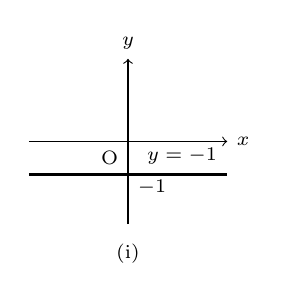
\begin{tikzpicture}[scale=0.42]
\ax{-3}{3}{-2.5}{2.5}
\draw[thick] (-3,-1)--(3,-1) node[above left]{\scriptsize $y=-1$};
\node[right] at (0,-1.4){\scriptsize $-1$};
\node at (0,-3.4){\scriptsize (i)};
\end{tikzpicture}\hfill
\begin{tikzpicture}[scale=0.42]
\ax{-3}{3}{-2.5}{2.5}
\draw[thick] (-2,-2.5)--(-2,2.5) node[above]{\scriptsize $x=-2$};
\node[below left] at (-2,0){\scriptsize $-2$};
\node at (0,-3.4){\scriptsize (ii)};
\end{tikzpicture}\hfill
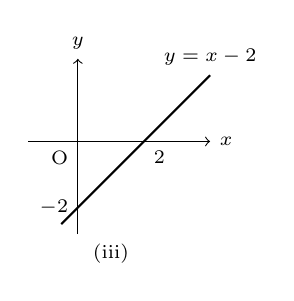
\begin{tikzpicture}[scale=0.42]
\ax{-1.5}{4}{-2.8}{2.5}
\draw[thick] (-0.5,-2.5)--(4,2) node[above]{\scriptsize $y=x-2$};
\node[left] at (0,-2){\scriptsize $-2$}; \node[below right] at (2,0){\scriptsize 2};
\node at (1,-3.4){\scriptsize (iii)};
\end{tikzpicture}\hfill
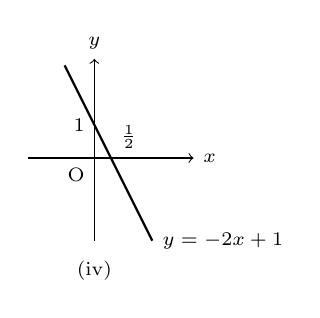
\begin{tikzpicture}[scale=0.42]
\ax{-2}{3}{-2.5}{3}
\draw[thick] (-0.9,2.8)--(1.75,-2.5) node[right]{\scriptsize $y=-2x+1$};
\node[left] at (0,1){\scriptsize 1}; \node[above right] at (0.5,0){\scriptsize $\frac12$};
\node at (0,-3.4){\scriptsize (iv)};
\end{tikzpicture}\\[4pt]
(iii)は傾き1，$y$ 切片 $-2$．(iv)は傾き $-2$，$y$ 切片 $1$．(ii)は $y$ 軸に平行な直線．\\[4pt]
(2)\ (i)\ $f(0)=|-2|+1=3$，\ $f(2)=0+1=1$，\ $f(5)=3+1=4$\\[2pt]
\hspace*{1.5em}(ii)\ $0\leqq x\leqq3$ より $-2\leqq x-2\leqq1$，よって $0\leqq|x-2|\leqq2$．\quad 値域は\quad $1\leqq f(x)\leqq3$\\
\hspace*{1.5em}\point{両端の値 $f(0)=3$，$f(3)=2$ だけで「$2\leqq f(x)\leqq3$」としてはいけない}
\end{kai}

\ans{27}{点の移動}
\begin{kai}
(1)\ $(2+3,\ -3-2)=(5,\ -5)$\qquad (2)\ $(2,\ 3)$\qquad (3)\ $(-2,\ -3)$\qquad (4)\ $(-2,\ 3)$\\
\point{$x$ 軸対称は $y$ 座標の符号，$y$ 軸対称は $x$ 座標の符号，原点対称は両方の符号が変わる}
\end{kai}

\ans{28}{平方完成}
\begin{kai}
(1)\ $y=-(x^2-4x)-1=-\{(x-2)^2-4\}-1=-(x-2)^2+3$\\[2pt]
(2)\ $y=3(x^2+2x)+1=3\{(x+1)^2-1\}+1=3(x+1)^2-2$
\end{kai}

\ans{29}{2次関数 $y=a(x-p)^2+q$ のグラフ}
\begin{kai}
(1)\ 下に凸，頂点 $(-2,\ -1)$，$y$ 切片 $3$\qquad
(2)\ $y=2(x+1)^2-3$．下に凸，頂点 $(-1,\ -3)$，$y$ 切片 $-1$\\[2pt]
(3)\ $y=-2\left(x^2-\dfrac52x\right)-2=-2\left(x-\dfrac54\right)^2+\dfrac98$．上に凸，頂点 $\left(\dfrac54,\ \dfrac98\right)$，$y$ 切片 $-2$\\[2pt]
(4)\ $y=\dfrac12(x^2+4x)+1=\dfrac12(x+2)^2-1$．下に凸，頂点 $(-2,\ -1)$，$y$ 切片 $1$\\[4pt]
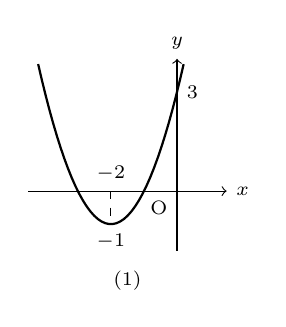
\begin{tikzpicture}[scale=0.42]
\ax{-4.5}{1.5}{-1.8}{4}
\draw[thick,domain=-4.2:0.2,samples=40] plot (\x,{(\x+2)^2-1});
\draw[dashed] (-2,0)--(-2,-1);
\node[above] at (-2,0){\scriptsize $-2$}; \node[right] at (0,3){\scriptsize 3};
\node[below] at (-2,-1){\scriptsize $-1$};
\node at (-1.5,-2.7){\scriptsize (1)};
\end{tikzpicture}\hfill
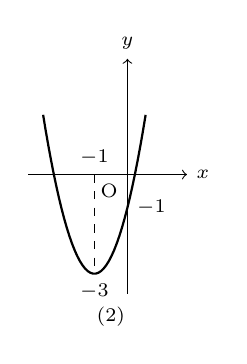
\begin{tikzpicture}[scale=0.42]
\ax{-3}{1.8}{-3.6}{3.5}
\draw[thick,domain=-2.55:0.55,samples=40] plot (\x,{2*(\x+1)^2-3});
\draw[dashed] (-1,0)--(-1,-3);
\node[above] at (-1,0){\scriptsize $-1$}; \node[right] at (0,-1){\scriptsize $-1$};
\node[below] at (-1,-3){\scriptsize $-3$};
\node at (-0.5,-4.3){\scriptsize (2)};
\end{tikzpicture}\hfill
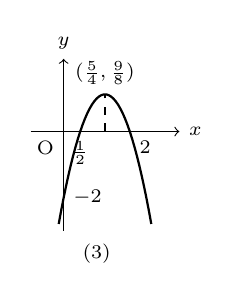
\begin{tikzpicture}[scale=0.42]
\ax{-1}{3.5}{-3}{2.2}
\draw[thick,domain=-0.15:2.65,samples=40] plot (\x,{-2*\x*\x+5*\x-2});
\draw[dashed] (1.25,0)--(1.25,1.125);
\node[right] at (0,-2){\scriptsize $-2$}; \node[above] at (1.25,1.125){\scriptsize $(\frac54,\frac98)$};
\node[below] at (0.5,0){\scriptsize $\frac12$}; \node[below right] at (2,0){\scriptsize 2};
\node at (1,-3.7){\scriptsize (3)};
\end{tikzpicture}\hfill
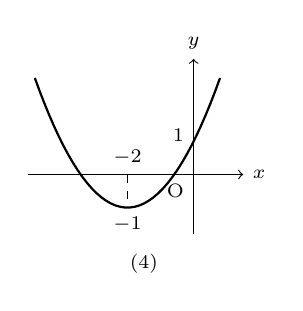
\begin{tikzpicture}[scale=0.42]
\ax{-5}{1.5}{-1.8}{3.5}
\draw[thick,domain=-4.8:0.8,samples=40] plot (\x,{0.5*(\x+2)^2-1});
\draw[dashed] (-2,0)--(-2,-1);
\node[above] at (-2,0){\scriptsize $-2$}; \node[left] at (0,1.2){\scriptsize 1};
\node[below] at (-2,-1){\scriptsize $-1$};
\node at (-1.5,-2.7){\scriptsize (4)};
\end{tikzpicture}
\end{kai}

\ans{30}{放物線の平行移動}
\begin{kai}
\point{$x^2$ の係数はそのままで，頂点を移動する}\\
(1)\ (i)\ $y=3(x-2)^2-3$\\
\hspace*{1.5em}(ii)\ $y=(x+2)^2-3$ より頂点は $(-2,\ -3)$．これを移動すると $(0,\ -6)$．\quad $y=x^2-6$\\[2pt]
(2)\ ①は $y=2(x-1)^2+1$ で頂点 $(1,\ 1)$．②は $y=2(x+2)^2-3$ で頂点 $(-2,\ -3)$．\\
\hspace*{1.5em}よって，②を $x$ 軸方向に $3$，$y$ 軸方向に $4$ だけ平行移動すると①になる．
\end{kai}

\ans{31}{放物線の対称移動}
\begin{kai}
$y=(x+3)^2-4$ より頂点は $(-3,\ -4)$，下に凸．\point{頂点を移動し，凸の向きも確認}\\
(i)\ 頂点 $(-3,\ 4)$，上に凸．\quad $y=-(x+3)^2+4$，すなわち $y=-x^2-6x-5$\\
(ii)\ 頂点 $(3,\ -4)$，下に凸．\quad $y=(x-3)^2-4$，すなわち $y=x^2-6x+5$\\
(iii)\ 頂点 $(3,\ 4)$，上に凸．\quad $y=-(x-3)^2+4$，すなわち $y=-x^2+6x-5$
\end{kai}

\ans{32}{放物線の移動}
\begin{kai}
\point{具体的にわかっている移動後の式から逆にたどる}\\
$y=-x^2+4x-1=-(x-2)^2+3$ より頂点 $(2,\ 3)$，上に凸．\\
これを $x$ 軸に関して対称移動すると，頂点 $(2,\ -3)$ で下に凸．\\
さらに $x$ 軸方向に $-3$ だけ平行移動すると，頂点 $(-1,\ -3)$ で下に凸の放物線 $y=(x+1)^2-3=x^2+2x-2$．\\
これが $y=x^2+ax+b$ と一致するので\quad $a=2$，$b=-2$
\end{kai}

\ans{33}{2次関数の決定}
\begin{kai}
(1)\ $y=a(x-1)^2-2$ とおく．$(3,\ 6)$ を通るので $6=4a-2$，$a=2$．\quad $y=2(x-1)^2-2$\\[2pt]
(2)\ $y=a(x+1)(x-3)$ とおく．$(0,\ 6)$ を通るので $6=-3a$，$a=-2$．\quad $y=-2(x+1)(x-3)$\\[2pt]
(3)\ $y=ax^2+bx+c$ とおく．$a-b+c=6$，$a+b+c=2$，$4a+2b+c=6$．\\
\hspace*{1.5em}第1式と第2式から $b=-2$，$a+c=4$．第3式は $4a+c=10$．よって $a=2$，$c=2$．\quad $y=2x^2-2x+2$\\[2pt]
(4)\ 2点 $(-2,\ 7)$，$(2,\ 7)$ を通るので，軸は $y$ 軸．$y=ax^2+c$ とおける．\\
\hspace*{1.5em}$4a+c=7$，$a+c=4$ より $a=1$，$c=3$．\quad $y=x^2+3$\\[2pt]
(5)\ 2点 $(0,\ 8)$，$(4,\ 8)$ を通るので軸は $x=2$．$x$ 軸に接するので頂点は $(2,\ 0)$．\\
\hspace*{1.5em}$y=a(x-2)^2$ とおく．$(0,\ 8)$ を通るので $a=2$．\quad $y=2(x-2)^2$
\end{kai}

\ans{34}{絶対値記号のついた関数のグラフ}
\begin{kai}
(1)\ $y=x+2$ のグラフの $x$ 軸より下の部分を折り返す．\\
(2)\ $y=\begin{cases}-2x+2 & (x<0)\\ 2 & (0\leqq x<2)\\ 2x-2 & (2\leqq x)\end{cases}$\\[2pt]
(3)\ $y=x^2-2x-3=(x-1)^2-4$ のグラフの $x$ 軸より下の部分を折り返す．$x$ 軸との交点は $x=-1,\ 3$．\\
(4)\ $y=\begin{cases}(x-1)^2-4 & (x\geqq0)\\ (x+1)^2-4 & (x<0)\end{cases}$\quad（$y$ 軸に関して対称なグラフ）\\[4pt]
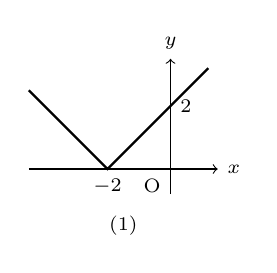
\begin{tikzpicture}[scale=0.4]
\ax{-4.5}{1.5}{-0.8}{3.5}
\draw[thick] (-4.5,2.5)--(-2,0)--(1.2,3.2);
\node[below] at (-2,0){\scriptsize $-2$}; \node[right] at (0,2){\scriptsize 2};
\node at (-1.5,-1.8){\scriptsize (1)};
\end{tikzpicture}\hfill
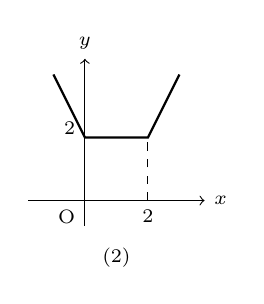
\begin{tikzpicture}[scale=0.4]
\ax{-1.8}{3.8}{-0.8}{4.5}
\draw[thick] (-1,4)--(0,2)--(2,2)--(3,4);
\draw[dashed] (2,0)--(2,2);
\node[left] at (0,2.3){\scriptsize 2}; \node[below] at (2,0){\scriptsize 2};
\node at (1,-1.8){\scriptsize (2)};
\end{tikzpicture}\hfill
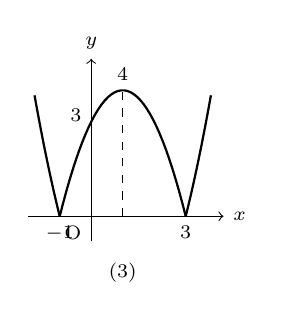
\begin{tikzpicture}[scale=0.4]
\ax{-2}{4.2}{-0.8}{5}
\draw[thick,domain=-1.8:-1,samples=20] plot (\x,{(\x-1)^2-4});
\draw[thick,domain=-1:3,samples=40] plot (\x,{4-(\x-1)^2});
\draw[thick,domain=3:3.8,samples=20] plot (\x,{(\x-1)^2-4});
\draw[dashed] (1,0)--(1,4);
\node[below] at (-1,0){\scriptsize $-1$}; \node[below] at (3,0){\scriptsize 3};
\node[above] at (1,4){\scriptsize 4}; \node[left] at (0,3.2){\scriptsize 3};
\node at (1,-1.8){\scriptsize (3)};
\end{tikzpicture}\hfill
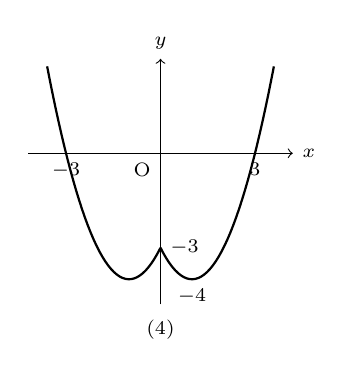
\begin{tikzpicture}[scale=0.4]
\ax{-4.2}{4.2}{-4.8}{3}
\draw[thick,domain=0:3.6,samples=40] plot (\x,{(\x-1)^2-4});
\draw[thick,domain=-3.6:0,samples=40] plot (\x,{(\x+1)^2-4});
\node[below] at (-3,0){\scriptsize $-3$}; \node[below] at (3,0){\scriptsize 3};
\node[right] at (0,-3){\scriptsize $-3$}; \node[below] at (1,-4){\scriptsize $-4$};
\node at (0,-5.6){\scriptsize (4)};
\end{tikzpicture}
\end{kai}

\ans{35}{最大・最小（Ⅰ）}
\begin{kai}
(1)\ 右下がりの直線だから，$x=-1$ のとき最大値 $5$，$x=2$ のとき最小値 $-4$\\[2pt]
(2)\ $y=\begin{cases}-x+3 & (0\leqq x<1)\\ 3x-1 & (1\leqq x\leqq3)\end{cases}$\quad グラフより $x=3$ のとき最大値 $8$，$x=1$ のとき最小値 $2$\\[2pt]
(3)\ $y=(x-2)^2-3$．頂点 $(2,\ -3)$ で下に凸．\point{両端と頂点の $y$ 座標を比べる}\\
\hspace*{1.5em}(i)\ 最大値なし，最小値 $-3$（$x=2$）\\
\hspace*{1.5em}(ii)\ 減少するので，最大値 $6$（$x=-1$），最小値 $-2$（$x=1$）\\
\hspace*{1.5em}(iii)\ 増加するので，最大値 $6$（$x=5$），最小値 $-2$（$x=3$）\\
\hspace*{1.5em}(iv)\ $y(1)=-2$，$y(4)=1$ より，最大値 $1$（$x=4$），最小値 $-3$（$x=2$）\\
\hspace*{1.5em}(v)\ $-3\leqq y<1$ より，最大値なし，最小値 $-3$（$x=2$）\\
\hspace*{1.5em}(vi)\ $1<y<6$ より，最大値，最小値ともになし
\end{kai}

\ans{36}{最大・最小（Ⅱ）}
\begin{kai}
$f(x)=(x-a)^2+3-a^2$．軸は $x=a$．\point{軸と定義域の位置関係で場合分け}\\
(1)\ $a<0$ のとき $m(a)=f(0)=3$，\quad $0\leqq a\leqq2$ のとき $m(a)=f(a)=3-a^2$，\quad $2<a$ のとき $m(a)=f(2)=7-4a$\\[2pt]
(2)\ \point{最大値は軸と定義域の中央 $x=1$ の位置関係で決まる}\\
\hspace*{1.5em}$a\leqq1$ のとき $M(a)=f(2)=7-4a$，\quad $1<a$ のとき $M(a)=f(0)=3$\\[2pt]
(3)\ $a<0$ では $m(a)=3$ で不適．$0\leqq a\leqq2$ では $3-a^2=-1$ より $a=2$（適する）．$2<a$ では $7-4a=-1$ より $a=2$ で不適．\quad $a=2$
\end{kai}

\ans{37}{最大・最小（Ⅲ）}
\begin{kai}
(1)\ $y=4-2x$．$y\geqq0$ より $0\leqq x\leqq2$．\point{消した文字の条件を残った文字に移す}\\
\hspace*{1.5em}$xy=x(4-2x)=-2(x-1)^2+2$．$x=1$，$y=2$ のとき最大値 $2$．\\
\hspace*{1.5em}$x^2+y^2=5x^2-16x+16=5\left(x-\dfrac85\right)^2+\dfrac{16}{5}$．$x=\dfrac85$，$y=\dfrac45$ のとき最小値 $\dfrac{16}5$\\[2pt]
(2)\ $t=(x+1)^2-1$ で $-2\leqq x\leqq1$ より $-1\leqq t\leqq3$．$y=t^2-2t+3=(t-1)^2+2$．\\
\hspace*{1.5em}最小値 $2$（$t=1$：$x^2+2x=1$，$-2\leqq x\leqq1$ より $x=-1+\sqrt2$）\\
\hspace*{1.5em}最大値 $6$（$t=-1$：$x=-1$，\ $t=3$：$x=1$）
\end{kai}

\ans{38}{最大・最小（Ⅳ）}
\begin{kai}
(1)\ \point{$x$ について整理して平方完成}\\
\hspace*{1.5em}$z=x^2-2(2y-1)x+5y^2-6y+4=\{x-(2y-1)\}^2-(2y-1)^2+5y^2-6y+4=\{x-(2y-1)\}^2+y^2-2y+3$\\
\hspace*{1.5em}よって\quad $m=y^2-2y+3$\\[2pt]
(2)\ $z=\{x-(2y-1)\}^2+(y-1)^2+2\geqq2$．等号は $x-(2y-1)=0$ かつ $y=1$，すなわち $x=1$，$y=1$ のとき．\\
\hspace*{1.5em}最小値 $2$（$x=1$，$y=1$）
\end{kai}

\ans{39}{最大・最小（Ⅴ）}
\begin{kai}
$\mathrm{AB}=\sqrt{6^2+8^2}=10$．\\
(1)\ DF $/\!/$ BC より $\mathrm{AD}:\mathrm{DF}=\mathrm{AB}:\mathrm{BC}=10:6$，\quad $\mathrm{DF}=\dfrac35x$\\
\hspace*{1.5em}DE $/\!/$ AC より $\mathrm{BD}:\mathrm{DE}=\mathrm{BA}:\mathrm{AC}=10:8$，\quad $\mathrm{DE}=\dfrac45(10-x)$\\
\hspace*{1.5em}$S=\mathrm{DF}\cdot\mathrm{DE}=\dfrac{12}{25}x(10-x)$\\[2pt]
(2)\ \point{図形の問題は変数に範囲がつく}\quad $0<x<10$．\quad $S=-\dfrac{12}{25}(x-5)^2+12$\\
\hspace*{1.5em}$x=5$ のとき最大値 $12$
\end{kai}

\ans{40}{2次方程式の解とその判別}
\begin{kai}
(1)\ (i)\ $x=-3\pm\sqrt{9+3}=-3\pm2\sqrt3$\\
\hspace*{1.5em}(ii)\ $(x^2-4)(x^2-9)=0$ より $x^2=4,\ 9$．\quad $x=\pm2,\ \pm3$\\
\hspace*{1.5em}(iii)\ $x^2+2x=t$ とおくと $t=(x+1)^2-1$ だから $t\geqq-1$．\\
\hspace*{1.5em}$(t-3)(t+2)-14=0$，$t^2-t-20=0$，$(t-5)(t+4)=0$．$t\geqq-1$ より $t=5$．\\
\hspace*{1.5em}$x^2+2x-5=0$ より\quad $x=-1\pm\sqrt6$\\[2pt]
(2)\ 判別式を $D$ とすると $\dfrac D4=9-k$．\\
\hspace*{1.5em}$k<9$ のとき異なる2つの実数解，$k=9$ のとき重解，$k>9$ のとき実数解をもたない．
\end{kai}

\ans{41}{放物線と $x$ 軸との位置関係}
\begin{kai}
\point{凸の向きと頂点の $y$ 座標の符号で判断}\\
(1)\ $y=(x-1)^2-4$．下に凸で頂点の $y$ 座標 $<0$．異なる2点で交わる．$(x+1)(x-3)=0$ より $x=-1,\ 3$\\[2pt]
(2)\ $y=-(x-3)^2+2$．上に凸で頂点の $y$ 座標 $>0$．異なる2点で交わる．$(x-3)^2=2$ より $x=3\pm\sqrt2$\\[2pt]
(3)\ $y=(x-3)^2$．頂点の $y$ 座標 $=0$ だから $x$ 軸と接する．接点の $x$ 座標は $3$\\[2pt]
(4)\ $y=-(x-1)^2-2$．上に凸で頂点の $y$ 座標 $<0$．$x$ 軸と共有点をもたない．
\end{kai}

\ans{42}{放物線と直線との位置関係}
\begin{kai}
\point{連立してできる2次方程式の判別式を調べる}\\
(1)\ $x^2-4x+5=2x$ より $x^2-6x+5=0$．$\dfrac D4=9-5=4>0$．\quad 共有点は2個\\[2pt]
(2)\ $x^2-4x+5=2x-4$ より $x^2-6x+9=0$．$\dfrac D4=9-9=0$．\quad 共有点は1個\\[2pt]
(3)\ $x^2-4x+5=-x+1$ より $x^2-3x+4=0$．$D=9-16=-7<0$．\quad 共有点は0個
\end{kai}

\ans{43}{放物線の接線}
\begin{kai}
$x^2+4x+1=-2x+a$ を整理して $x^2+6x+(1-a)=0$ ……①\\
接するのは①が重解をもつときで，$\dfrac D4=9-(1-a)=8+a=0$．\quad $a=-8$\\
（このとき①は $(x+3)^2=0$ で，接点は $(-3,\ -2)$．）
\end{kai}

\ans{44}{2次不等式}
\begin{kai}
(1)\ $(x-1)(x-4)<0$ より\quad $1<x<4$\\[2pt]
(2)\ $x^2+4x+1=0$ の解は $x=-2\pm\sqrt3$．\quad $x\leqq-2-\sqrt3,\ -2+\sqrt3\leqq x$\\[2pt]
(3)\ $(3x+1)^2\leqq0$ より\quad $x=-\dfrac13$\\[2pt]
(4)\ $x^2+4x+5>0$，$(x+2)^2+1>0$ はつねに成り立つ．\quad すべての実数\\[2pt]
(5)\ \point{$x^2$ の係数を正にする（向きが変わる）}\quad $3x^2-5x-2<0$，$(3x+1)(x-2)<0$．\quad $-\dfrac13<x<2$\\[2pt]
(6)\ 第1式は $x(x-2)\leqq0$ より $0\leqq x\leqq2$．第2式は $(2x-1)(x-3)>0$ より $x<\dfrac12,\ 3<x$．\\
\hspace*{1.5em}共通部分をとって\quad $0\leqq x<\dfrac12$
\end{kai}

\ans{45}{係数の符号}
\begin{kai}
(1)\ 上に凸だから $a<0$\\
(2)\ 軸 $x=-\dfrac{b}{2a}<0$ で $a<0$ だから $b<0$\\
(3)\ $y$ 切片が正だから $c>0$\\
(4)\ $x$ 軸と2点で交わるから $b^2-4ac>0$\\
(5)\ $x=1$ のとき $y>0$ だから $a+b+c>0$\\
(6)\ $x=2$ のとき $y<0$ だから $4a+2b+c<0$\\
(7)\ $x=-1$ のとき $y>0$ だから $a-b+c>0$
\end{kai}

\ans{46}{解の配置}
\begin{kai}
$f(x)=x^2+2ax+a+2=(x+a)^2-a^2+a+2$．軸は $x=-a$．\\
(1)\ \point{判別式（頂点の $y$ 座標），軸の位置，端点の $y$ の符号}\\
\hspace*{1.5em}$\dfrac D4=a^2-a-2>0$ より $a<-1,\ 2<a$．軸 $-a>0$ より $a<0$．$f(0)=a+2>0$ より $a>-2$．\quad $-2<a<-1$\\[2pt]
(2)\ $f(0)=a+2<0$ より\quad $a<-2$\\[2pt]
(3)\ $\dfrac D4>0$ より $a<-1,\ 2<a$．軸 $-a>-1$ より $a<1$．$f(-1)=3-a>0$ より $a<3$．\quad $a<-1$
\end{kai}

\ans{47}{絶対不等式（Ⅰ）}
\begin{kai}
$f(x)=2x+a\ (x\geqq2)$ は増加するので最小値は $f(2)=4+a$．\\
\point{最小値 $\geqq0$}\quad $4+a\geqq0$ より\quad $a\geqq-4$
\end{kai}

\ans{48}{絶対不等式（Ⅱ）}
\begin{kai}
$f(x)=(x+a)^2-a^2+2a+8$．すべての $x$ で $f(x)>0$ となる条件は，頂点の $y$ 座標が正であること．\\
$-a^2+2a+8>0$，$a^2-2a-8<0$，$(a+2)(a-4)<0$．\quad $-2<a<4$\\
（別解：$x^2+2ax+2a+8=0$ の判別式 $\dfrac D4=a^2-2a-8<0$ としても同じ．）
\end{kai}

\ans{49}{文字係数の2次不等式}
\begin{kai}
(1)\ ①は $(x-2)(x-a)<0$．\point{2と $a$ の大小で場合分け}\\
\hspace*{1.5em}$a<2$ のとき $a<x<2$，\quad $a=2$ のとき $(x-2)^2<0$ で解なし，\quad $a>2$ のとき $2<x<a$\\[2pt]
(2)\ $a>2$ のとき，整数解が 3，4 の2個となるのは\quad $4<a\leqq5$\\
\hspace*{1.5em}$a<2$ のとき，整数解が 1，0 の2個となるのは\quad $-1\leqq a<0$\\
\hspace*{1.5em}よって\quad $-1\leqq a<0,\ 4<a\leqq5$
\end{kai}

\ans{50}{絶対値記号のついた2次方程式}
\begin{kai}
(1)\ \point{$x^2=|x|^2$}\quad $|x|^2-3|x|-4=0$，$(|x|+1)(|x|-4)=0$．$|x|\geqq0$ より $|x|=4$．\quad $x=\pm4$\\[2pt]
(2)\ $x^2-x-6=(x+2)(x-3)$ だから\\
\hspace*{1.5em}(i)\ $x\leqq-2,\ 3\leqq x$ のとき：②は $x^2-x-6=2x+4$，$x^2-3x-10=0$，$(x+2)(x-5)=0$．\\
\hspace*{1.5em}\hspace*{1.5em}$x=-2,\ 5$ はともに適する．\\
\hspace*{1.5em}(ii)\ $-2<x<3$ のとき：②は $-(x^2-x-6)=2x+4$，$x^2+x-2=0$，$(x+2)(x-1)=0$．\\
\hspace*{1.5em}\hspace*{1.5em}$-2<x<3$ より $x=1$．\\
\hspace*{1.5em}(i)，(ii)より\quad $x=-2,\ 1,\ 5$
\end{kai}

\ans{51}{絶対値記号のついた2次不等式}
\begin{kai}
(1)\ $|x|^2-|x|-6\leqq0$，$(|x|+2)(|x|-3)\leqq0$．$|x|+2>0$ より $|x|\leqq3$．\quad $-3\leqq x\leqq3$\\[2pt]
(2)\ $x^2+4x+3=(x+1)(x+3)$ だから\\
\hspace*{1.5em}(i)\ $x\leqq-3,\ -1\leqq x$ のとき：$x^2+4x+3<2x+5$，$x^2+2x-2<0$，$-1-\sqrt3<x<-1+\sqrt3$．\\
\hspace*{1.5em}\hspace*{1.5em}$-1-\sqrt3>-3$ に注意して，範囲と合わせると\quad $-1\leqq x<-1+\sqrt3$\\
\hspace*{1.5em}(ii)\ $-3<x<-1$ のとき：$-(x^2+4x+3)<2x+5$，$x^2+6x+8>0$，$(x+2)(x+4)>0$，$x<-4,\ -2<x$．\\
\hspace*{1.5em}\hspace*{1.5em}範囲と合わせると\quad $-2<x<-1$\\
\hspace*{1.5em}(i)，(ii)より\quad $-2<x<-1+\sqrt3$
\end{kai}

\shouans{第4章}{図形の性質}
\ans{52}{三角形の重心，外心，内心，垂心}
\begin{kai}
(1)\ 外心\qquad (2)\ 内心\qquad (3)\ 重心\qquad (4)\ 垂心\\
外接円の中心は外心，内接円の中心は内心．\\
\point{重心：3中線の交点\quad 外心：3辺の垂直2等分線の交点\quad 内心：3内角の2等分線の交点\quad 垂心：3垂線の交点}
\end{kai}

\ans{53}{角の2等分線の性質}
\begin{kai}
(1)\ \point{$\mathrm{BD}:\mathrm{DC}=\mathrm{AB}:\mathrm{AC}$}\quad $\mathrm{BD}:\mathrm{DC}=6:4=3:2$\\[2pt]
(2)\ $\mathrm{BD}=5\times\dfrac35=3$．$\triangle\mathrm{ABD}$ で BI は $\angle\mathrm B$ の2等分線だから\quad $\mathrm{AI}:\mathrm{ID}=\mathrm{BA}:\mathrm{BD}=6:3=2:1$\\[2pt]
(3)\ $\mathrm{AE}:\mathrm{EC}=\mathrm{BA}:\mathrm{BC}=6:5$ より $\mathrm{AE}=4\times\dfrac6{11}=\dfrac{24}{11}$．\\
\hspace*{1.5em}$\triangle\mathrm{ABE}$ で AI は $\angle\mathrm A$ の2等分線だから\quad $\mathrm{BI}:\mathrm{IE}=\mathrm{AB}:\mathrm{AE}=6:\dfrac{24}{11}=11:4$
\end{kai}

\ans{54}{チェバの定理}
\begin{kai}
チェバの定理より\quad $\dfrac{\mathrm{AF}}{\mathrm{FB}}\cdot\dfrac{\mathrm{BD}}{\mathrm{DC}}\cdot\dfrac{\mathrm{CE}}{\mathrm{EA}}=1$，\quad
$\dfrac{\mathrm{AF}}{\mathrm{FB}}\cdot\dfrac23\cdot\dfrac43=1$，\quad $\dfrac{\mathrm{AF}}{\mathrm{FB}}=\dfrac98$\\
よって\quad $\mathrm{AF}:\mathrm{FB}=9:8$
\end{kai}

\ans{55}{メネラウスの定理}
\begin{kai}
(1)\ $\triangle\mathrm{ABD}$ と直線 EC にメネラウスの定理を用いて\quad
$\dfrac{\mathrm{AE}}{\mathrm{EB}}\cdot\dfrac{\mathrm{BC}}{\mathrm{CD}}\cdot\dfrac{\mathrm{DP}}{\mathrm{PA}}=1$，\quad
$\dfrac12\cdot\dfrac31\cdot\dfrac{\mathrm{DP}}{\mathrm{PA}}=1$\\
\hspace*{1.5em}$\dfrac{\mathrm{DP}}{\mathrm{PA}}=\dfrac23$．\quad よって\quad $\mathrm{AP}:\mathrm{PD}=3:2$\\[2pt]
(2)\ \point{高さが共通な三角形の面積比は底辺の比}\\
\hspace*{1.5em}$\triangle\mathrm{ADC}=\dfrac13\triangle\mathrm{ABC}$，\quad $\triangle\mathrm{PDC}=\dfrac25\triangle\mathrm{ADC}=\dfrac25\cdot\dfrac13\triangle\mathrm{ABC}=\dfrac{2}{15}\triangle\mathrm{ABC}$\\
\hspace*{1.5em}よって\quad $\triangle\mathrm{PDC}:\triangle\mathrm{ABC}=2:15$
\end{kai}

\ans{56}{円周角}
\begin{kai}
(1)\ \point{同じ弧に対する円周角は等しい}\quad $\angle\mathrm{ACD}=\angle\mathrm{ABD}=40^\circ$（弧 AD），\quad $\angle\mathrm{BAC}=\angle\mathrm{BDC}=25^\circ$（弧 BC）\\[2pt]
(2)\ 中心角は円周角の2倍だから\quad $\angle\mathrm{AOD}=2\angle\mathrm{ABD}=80^\circ$\\[2pt]
(3)\ $\triangle\mathrm{ABP}$ で $\angle\mathrm{BAP}=25^\circ$，$\angle\mathrm{ABP}=40^\circ$ より\quad $\angle\mathrm{APB}=180^\circ-65^\circ=115^\circ$\\[2pt]
(4)\ $\triangle\mathrm{ABP}$ と $\triangle\mathrm{DCP}$ において，$\angle\mathrm{BAP}=\angle\mathrm{CDP}$（弧 BC に対する円周角），$\angle\mathrm{APB}=\angle\mathrm{DPC}$（対頂角）．\\
\hspace*{1.5em}2角がそれぞれ等しいので\quad $\triangle\mathrm{ABP}\backsim\triangle\mathrm{DCP}$
\end{kai}

\ans{57}{接弦定理}
\begin{kai}
(1)\ \point{接線と弦のつくる角は，その角の内部にある弧に対する円周角に等しい}\quad $\angle\mathrm{ACB}=\angle\mathrm{TAB}=55^\circ$\\[2pt]
(2)\ $\angle\mathrm{BAC}=180^\circ-(70^\circ+55^\circ)=55^\circ$\\[2pt]
(3)\ $\angle\mathrm{BAC}=\angle\mathrm{BCA}=55^\circ$ だから，$\mathrm{BA}=\mathrm{BC}$ の二等辺三角形
\end{kai}

\ans{58}{方べきの定理}
\begin{kai}
(1)\ $\triangle\mathrm{OAC}$ と $\triangle\mathrm{ODB}$ において，$\angle\mathrm{AOC}=\angle\mathrm{DOB}$（共通）．\\
\hspace*{1.5em}四角形 ABDC は円に内接しているので $\angle\mathrm{OAC}=180^\circ-\angle\mathrm{CAB}=\angle\mathrm{CDB}=\angle\mathrm{ODB}$．\\
\hspace*{1.5em}2角がそれぞれ等しいので\quad $\triangle\mathrm{OAC}\backsim\triangle\mathrm{ODB}$\\[2pt]
(2)\ (1)より $\mathrm{OA}:\mathrm{OC}=\mathrm{OD}:\mathrm{OB}$，すなわち $\mathrm{OA}\cdot\mathrm{OB}=\mathrm{OC}\cdot\mathrm{OD}$．\\
\hspace*{1.5em}$\mathrm{CD}=x$ とおくと $\mathrm{OD}=4+x$．$3\cdot8=4(4+x)$ より $x=2$．\quad $\mathrm{CD}=2$
\end{kai}

\ans{59}{2円の位置関係}
\begin{kai}
\point{接するときは中心と接点を結ぶ．円どうしなら中心どうしを結ぶ}\\
(1)\ A を通り直線 $\mathrm T_1\mathrm T_2$ に平行な直線と直線 $\mathrm{BT}_2$ の交点を H とすると，$\mathrm{BH}=9-4=5$．\\
\hspace*{1.5em}外接しているので $\mathrm{AB}=4+9=13$．$\mathrm T_1\mathrm T_2=\mathrm{AH}=\sqrt{13^2-5^2}=12$\\[2pt]
(2)\ 同様に $\mathrm{BH}=b-a$，$\mathrm{AB}=a+b$ だから\\
\hspace*{1.5em}$\mathrm T_1\mathrm T_2{}^2=(a+b)^2-(b-a)^2=4ab$．\quad $\mathrm T_1\mathrm T_2=2\sqrt{ab}$
\end{kai}

\ans{60}{平面幾何（Ⅰ）}
\begin{kai}
(1)\ $\triangle\mathrm{ABC}$ と直線 DF にメネラウスの定理を用いて\quad $\dfrac{\mathrm{AD}}{\mathrm{DB}}\cdot\dfrac{\mathrm{BF}}{\mathrm{FC}}\cdot\dfrac{\mathrm{CE}}{\mathrm{EA}}=1$\\
\hspace*{1.5em}$\dfrac32\cdot\dfrac{\mathrm{BF}}{\mathrm{FC}}\cdot\dfrac21=1$ より $\dfrac{\mathrm{BF}}{\mathrm{FC}}=\dfrac13$．\quad $\mathrm{BF}:\mathrm{FC}=1:3$（F は辺 CB の B 側の延長上）\\[2pt]
(2)\ \point{4点が同一円周上 → 方べきの定理}\quad $\mathrm{AD}\cdot\mathrm{AB}=\mathrm{AE}\cdot\mathrm{AC}$．\\
\hspace*{1.5em}$\mathrm{AD}=6$，$\mathrm{AE}=\dfrac13\mathrm{AC}$ だから $60=\dfrac13\mathrm{AC}^2$，$\mathrm{AC}^2=180$．\quad $\mathrm{AC}=6\sqrt5$
\end{kai}

\ans{61}{平面幾何（Ⅱ）}
\begin{kai}
(1)\ $\mathrm{BC}=\sqrt{36+64}=10$．面積を2通りに表して $\dfrac12\cdot6\cdot8=\dfrac12\cdot10\cdot\mathrm{AH}$，\quad $\mathrm{AH}=\dfrac{24}{5}$\\
\hspace*{1.5em}$\triangle\mathrm{ABH}\backsim\triangle\mathrm{CBA}$ より $\mathrm{BH}=\dfrac{\mathrm{AB}^2}{\mathrm{BC}}=\dfrac{36}{10}=\dfrac{18}{5}$\\[2pt]
(2)\ $\angle\mathrm{BAC}=90^\circ$ だから，A は BC を直径とする円周上にある．その中心は BC の中点 M だから，M は外心．\quad $\mathrm{AM}=\dfrac12\mathrm{BC}=5$\\[2pt]
(3)\ $\mathrm{HM}=\mathrm{BM}-\mathrm{BH}=5-\dfrac{18}{5}=\dfrac75$．\quad $\triangle\mathrm{AHM}=\dfrac12\cdot\dfrac75\cdot\dfrac{24}{5}=\dfrac{84}{25}$
\end{kai}

\ans{62}{四角形への応用（トレミーの定理）}
\begin{kai}
(1)\ AC は直径だから $\angle\mathrm{ABC}=\angle\mathrm{ADC}=90^\circ$．\quad $\mathrm{BC}=\mathrm{CD}=\sqrt{25-9}=4$\\[2pt]
(2)\ $3\cdot4+4\cdot3=5\cdot\mathrm{BD}$ より\quad $\mathrm{BD}=\dfrac{24}{5}$\\[2pt]
(3)\ $\mathrm{AB}=\mathrm{AD}$，$\mathrm{CB}=\mathrm{CD}$ だから，AC は BD の垂直二等分線．交点を K とすると BK は直角三角形 ABC の斜辺 AC への垂線．\\
\hspace*{1.5em}$\dfrac12\cdot3\cdot4=\dfrac12\cdot5\cdot\mathrm{BK}$ より $\mathrm{BK}=\dfrac{12}5$．\quad $\mathrm{BD}=2\mathrm{BK}=\dfrac{24}{5}$ で一致する．
\end{kai}

\ans{63}{内接球・外接球}
\begin{kai}
\point{球の中心と接点を含む平面（円錐の軸を含む平面）で切る}\\
断面の二等辺三角形を ABC（A が頂点），底面の中心を D，球の中心を O，AB と球の接点を E とする．$\mathrm{AB}=\sqrt{5^2+12^2}=13$．\\
(1)\ $\triangle\mathrm{ABD}\backsim\triangle\mathrm{AOE}$ より $\mathrm{AB}:\mathrm{BD}=\mathrm{AO}:\mathrm{OE}$，$13:5=(12-R):R$．\\
\hspace*{1.5em}$13R=60-5R$ より\quad $R=\dfrac{10}{3}$\\[2pt]
(2)\ $\mathrm{AO}=12-\dfrac{10}3=\dfrac{26}3$，\quad $\mathrm{AE}=\sqrt{\left(\dfrac{26}3\right)^2-\left(\dfrac{10}3\right)^2}=8$．\\
\hspace*{1.5em}AC と球の接点を F とすると，$\triangle\mathrm{AEF}\backsim\triangle\mathrm{ABC}$ で相似比は $8:13$．$\mathrm{EF}=10\times\dfrac{8}{13}=\dfrac{80}{13}$．\\
\hspace*{1.5em}求める円の半径は\quad $r=\dfrac12\mathrm{EF}=\dfrac{40}{13}$
\end{kai}

\ans{64}{特殊な四面体（Ⅰ）}
\begin{kai}
(1)\ $\triangle\mathrm{OAH}$，$\triangle\mathrm{OBH}$，$\triangle\mathrm{OCH}$ は，OH が共通，$\angle\mathrm{OHA}=\angle\mathrm{OHB}=\angle\mathrm{OHC}=90^\circ$，$\mathrm{OA}=\mathrm{OB}=\mathrm{OC}$ の直角三角形なので合同．\\
\hspace*{1.5em}よって $\mathrm{HA}=\mathrm{HB}=\mathrm{HC}$ となり，H は $\triangle\mathrm{ABC}$ の外心．\\[2pt]
(2)\ 正弦定理より $2\mathrm{AH}=\dfrac{6}{\sin60^\circ}$，\quad $\mathrm{AH}=2\sqrt3$．\quad $\mathrm{OH}=\sqrt{25-12}=\sqrt{13}$\\[2pt]
(3)\ $\triangle\mathrm{ABC}=\dfrac{\sqrt3}4\cdot6^2=9\sqrt3$．\quad $V=\dfrac13\cdot9\sqrt3\cdot\sqrt{13}=3\sqrt{39}$
\end{kai}

\ans{65}{特殊な四面体（Ⅱ）}
\begin{kai}
(1)\ 垂線の足を G とすると，類題64と同様に G は正三角形 BCD の外心．$\mathrm{BG}=\dfrac{6}{2\sin60^\circ}=2\sqrt3$．\\
\hspace*{1.5em}$h=\mathrm{AG}=\sqrt{36-12}=2\sqrt6$\\[2pt]
(2)\ $\triangle\mathrm{BCD}=9\sqrt3$．\quad $V=\dfrac13\cdot9\sqrt3\cdot2\sqrt6=18\sqrt2$\\[2pt]
(3)\ \point{内心 I と4頂点を結んで4つの四面体に分ける}\quad $V=\dfrac13r\times(4\times9\sqrt3)=12\sqrt3\,r$．\\
\hspace*{1.5em}$12\sqrt3\,r=18\sqrt2$ より\quad $r=\dfrac{3\sqrt2}{2\sqrt3}=\dfrac{\sqrt6}{2}$
\end{kai}


\shouans{第5章}{図形と計量}
\ans{66}{鋭角の三角比}
\begin{kai}
(1)\ 斜辺は $\sqrt{15^2+8^2}=17$．\quad $\sin\theta=\dfrac8{17}$，$\cos\theta=\dfrac{15}{17}$，$\tan\theta=\dfrac8{15}$\\[2pt]
(2)\ 底辺は $\sqrt{25^2-7^2}=24$．\quad $\sin\theta=\dfrac7{25}$，$\cos\theta=\dfrac{24}{25}$，$\tan\theta=\dfrac7{24}$\\
\point{角 $\theta$ を左下，直角を右下にした図で考える}
\end{kai}

\ans{67}{有名角の三角比}
\begin{kai}
(1)\ $\left(\dfrac{\sqrt3}2\right)^2=\dfrac34$\qquad
(2)\ $2\cdot\dfrac1{\sqrt2}-4\cdot\dfrac12=\sqrt2-2$\\[2pt]
(3)\ $\dfrac1{\sqrt3}+\dfrac{\sqrt3}2=\dfrac{\sqrt3}3+\dfrac{\sqrt3}2=\dfrac{5\sqrt3}{6}$\qquad
(4)\ $\dfrac12\cdot\dfrac{\sqrt3}2+\dfrac{\sqrt3}2\cdot\dfrac12=\dfrac{\sqrt3}2$
\end{kai}

\ans{68}{鈍角の三角比}
\begin{kai}
\point{半径 $r$ の半円上の点 $\mathrm P(x,\ y)$ で $\sin\theta=\dfrac yr$，$\cos\theta=\dfrac xr$，$\tan\theta=\dfrac yx$}\\
(1)\ 半径2の半円で $150^\circ$ の点は $\mathrm P(-\sqrt3,\ 1)$．\quad $\cos150^\circ=-\dfrac{\sqrt3}2$\\[2pt]
(2)\ 半径 $\sqrt2$ の半円で $135^\circ$ の点は $\mathrm P(-1,\ 1)$．\quad $\sin135^\circ=\dfrac1{\sqrt2}$\\[2pt]
(3)\ 半径2の半円で $120^\circ$ の点は $\mathrm P(-1,\ \sqrt3)$．\quad $\tan120^\circ=\dfrac{\sqrt3}{-1}=-\sqrt3$
\end{kai}

\ans{69}{補角・余角の三角比}
\begin{kai}
(1)\ $\sin150^\circ=\sin(180^\circ-30^\circ)=\sin30^\circ=\dfrac12$\\[2pt]
(2)\ $\cos120^\circ=\cos(180^\circ-60^\circ)=-\cos60^\circ=-\dfrac12$\\[2pt]
(3)\ $\tan135^\circ=\tan(180^\circ-45^\circ)=-\tan45^\circ=-1$
\end{kai}

\ans{70}{三角比の相互関係}
\begin{kai}
(1)\ $\sin^2\theta=1-\dfrac49=\dfrac59$．$\sin\theta\geqq0$ より $\sin\theta=\dfrac{\sqrt5}3$，\quad $\tan\theta=\dfrac{\sin\theta}{\cos\theta}=-\dfrac{\sqrt5}{2}$\\[2pt]
(2)\ $\dfrac1{\cos^2\theta}=1+\tan^2\theta=5$．\point{$\tan\theta<0$ だから $\theta$ は鈍角，$\cos\theta<0$}\\
\hspace*{1.5em}$\cos\theta=-\dfrac1{\sqrt5}=-\dfrac{\sqrt5}5$，\quad $\sin\theta=\tan\theta\cos\theta=\dfrac2{\sqrt5}=\dfrac{2\sqrt5}5$\\[2pt]
(3)\ $\cos^2\theta=1-\dfrac{25}{169}=\dfrac{144}{169}$．\point{$\theta$ は鋭角とも鈍角ともありうる}\\
\hspace*{1.5em}$\cos\theta=\pm\dfrac{12}{13}$，\quad $\tan\theta=\pm\dfrac{5}{12}$（複号同順）
\end{kai}

\ans{71}{三角比の計算（Ⅰ）}
\begin{kai}
(1)\ $(\sin^2\theta+2\sin\theta\cos\theta+\cos^2\theta)+(\sin^2\theta-2\sin\theta\cos\theta+\cos^2\theta)=2(\sin^2\theta+\cos^2\theta)=2$\\[2pt]
(2)\ \point{$\tan\theta$ を $\sin\theta$，$\cos\theta$ で表す}\quad
$\dfrac{\sin\theta}{1+\cos\theta}+\dfrac{\cos\theta}{\sin\theta}=\dfrac{\sin^2\theta+\cos\theta+\cos^2\theta}{(1+\cos\theta)\sin\theta}=\dfrac{1+\cos\theta}{(1+\cos\theta)\sin\theta}=\dfrac1{\sin\theta}$
\end{kai}

\ans{72}{三角比の計算（Ⅱ）}
\begin{kai}
(1)\ $(\sin\theta-\cos\theta)^2=1-2\sin\theta\cos\theta$ だから $\dfrac14=1-2\sin\theta\cos\theta$．\quad $\sin\theta\cos\theta=\dfrac38$\\[2pt]
(2)\ $\sin^3\theta-\cos^3\theta=(\sin\theta-\cos\theta)(\sin^2\theta+\sin\theta\cos\theta+\cos^2\theta)=\dfrac12\left(1+\dfrac38\right)=\dfrac{11}{16}$
\end{kai}

\ans{73}{三角方程式（Ⅰ）}
\begin{kai}
(1)\ (i)\ $\cos\theta=\dfrac12$ より\quad $\theta=60^\circ$\qquad
(ii)\ $\sin\theta=\dfrac1{\sqrt2}$ より\quad $\theta=45^\circ,\ 135^\circ$\\[2pt]
\hspace*{1.5em}(iii)\ $\tan\theta=-\sqrt3$ より\quad $\theta=120^\circ$\\[2pt]
(2)\ \point{$0^\circ\leqq2\theta\leqq180^\circ$ で $2\theta$ を求めてから2で割る}\\
\hspace*{1.5em}(i)\ $\cos2\theta=-\dfrac12$ より $2\theta=120^\circ$．\quad $\theta=60^\circ$\\[2pt]
\hspace*{1.5em}(ii)\ $\sin2\theta=\dfrac{\sqrt3}2$ より $2\theta=60^\circ,\ 120^\circ$．\quad $\theta=30^\circ,\ 60^\circ$\\[2pt]
\hspace*{1.5em}(iii)\ $\tan2\theta=\dfrac1{\sqrt3}$ より $2\theta=30^\circ$．\quad $\theta=15^\circ$
\end{kai}

\ans{74}{三角不等式（Ⅰ）}
\begin{kai}
\point{方程式を解いて境界の角を求め，単位円で範囲を読む}\\
(1)\ (i)\ $\cos\theta\geqq\dfrac12$ より\quad $0^\circ\leqq\theta\leqq60^\circ$\\[2pt]
\hspace*{1.5em}(ii)\ $\sin\theta<\dfrac{\sqrt3}2$ より\quad $0^\circ\leqq\theta<60^\circ,\ 120^\circ<\theta\leqq180^\circ$\\[2pt]
\hspace*{1.5em}(iii)\ $\tan\theta\geqq1$ より\quad $45^\circ\leqq\theta<90^\circ$\quad（$\tan90^\circ$ は定義されない）\\[2pt]
(2)\ (i)\ $\cos2\theta>\dfrac12$，$0^\circ\leqq2\theta\leqq180^\circ$ より $0^\circ\leqq2\theta<60^\circ$．\quad $0^\circ\leqq\theta<30^\circ$\\[2pt]
\hspace*{1.5em}(ii)\ $\sin2\theta\geqq\dfrac{\sqrt3}2$ より $60^\circ\leqq2\theta\leqq120^\circ$．\quad $30^\circ\leqq\theta\leqq60^\circ$\\[2pt]
\hspace*{1.5em}(iii)\ $\tan2\theta<-\sqrt3$ より $90^\circ<2\theta<120^\circ$．\quad $45^\circ<\theta<60^\circ$
\end{kai}

\ans{75}{三角方程式（Ⅱ）}
\begin{kai}
(1)\ \point{$\sin x$ に統一する}\quad $2(1-\sin^2x)-3\sin x=0$，$2\sin^2x+3\sin x-2=0$．\\
\hspace*{1.5em}$\sin x=t$ とおくと $0\leqq t\leqq1$．$(2t-1)(t+2)=0$ より $t=\dfrac12$．\quad $\sin x=\dfrac12$\\[2pt]
(2)\ $0^\circ\leqq x\leqq180^\circ$ だから\quad $x=30^\circ,\ 150^\circ$
\end{kai}

\ans{76}{三角不等式（Ⅱ）}
\begin{kai}
(1)\ $2(1-\cos^2x)+\cos x>2$ より $2\cos^2x-\cos x<0$．\\
\hspace*{1.5em}$\cos x=t$ とおくと $-1\leqq t\leqq1$．$t(2t-1)<0$ より $0<t<\dfrac12$．\quad $0<\cos x<\dfrac12$\\[2pt]
(2)\ 単位円より\quad $60^\circ<x<90^\circ$
\end{kai}

\ans{77}{最大値・最小値}
\begin{kai}
(1)\ $y=(1-\sin^2x)+\sin x$ より\quad $y=-t^2+t+1$\\[2pt]
(2)\ $0^\circ\leqq x\leqq180^\circ$ だから\quad $0\leqq t\leqq1$\\[2pt]
(3)\ $y=-\left(t-\dfrac12\right)^2+\dfrac54$．$0\leqq t\leqq1$ において\\
\hspace*{1.5em}$t=\dfrac12$，すなわち $x=30^\circ,\ 150^\circ$ のとき最大値 $\dfrac54$\\
\hspace*{1.5em}$t=0,\ 1$，すなわち $x=0^\circ,\ 90^\circ,\ 180^\circ$ のとき最小値 $1$
\end{kai}

\ans{78}{正弦定理}
\begin{kai}
(1)\ $\angle\mathrm B=180^\circ-(75^\circ+60^\circ)=45^\circ$．正弦定理より $\dfrac{\mathrm{AB}}{\sin60^\circ}=\dfrac{3}{\sin45^\circ}$．\\
\hspace*{1.5em}$\mathrm{AB}=3\cdot\dfrac{\sqrt3}2\cdot\sqrt2=\dfrac{3\sqrt6}2$\\[2pt]
(2)\ $2R=\dfrac3{\sin45^\circ}=3\sqrt2$．\quad $R=\dfrac{3\sqrt2}{2}$
\end{kai}

\ans{79}{余弦定理}
\begin{kai}
$\mathrm{AB}^2=2^2+3^2-2\cdot2\cdot3\cos60^\circ=7$．\quad $\mathrm{AB}=\sqrt7$\\
\point{2辺とその間の角 → 余弦定理}
\end{kai}

\ans{80}{正弦定理・余弦定理の使い分け}
\begin{kai}
(1)\ \point{2辺と1角（間の角でない）→ 余弦定理で方程式}\quad $\mathrm{BC}=x$ とすると $7^2=5^2+x^2-2\cdot5\cdot x\cos60^\circ$．\\
\hspace*{1.5em}$x^2-5x-24=0$，$(x-8)(x+3)=0$，$x>0$ より\quad $\mathrm{BC}=8$\\[2pt]
(2)\ 正弦定理より $\dfrac{5}{\sin C}=\dfrac{7}{\sin60^\circ}$．\quad $\sin C=\dfrac{5}{7}\cdot\dfrac{\sqrt3}{2}=\dfrac{5\sqrt3}{14}$\\[2pt]
(3)\ $2R=\dfrac{7}{\sin60^\circ}=\dfrac{14}{\sqrt3}$．\quad $R=\dfrac{7\sqrt3}{3}$
\end{kai}

\ans{81}{中線定理}
\begin{kai}
(1)\ $\triangle\mathrm{ABC}$ に余弦定理を用いて\quad $\cos C=\dfrac{(2a)^2+b^2-c^2}{2\cdot2a\cdot b}=\dfrac{4a^2+b^2-c^2}{4ab}$\\[2pt]
(2)\ \point{$\angle\mathrm C$ を $\triangle\mathrm{AMC}$ の内角として2度使う}\\
\hspace*{1.5em}$\mathrm{AM}^2=b^2+a^2-2ab\cos C=a^2+b^2-\dfrac{4a^2+b^2-c^2}{2}=\dfrac{b^2+c^2-2a^2}{2}$\\[2pt]
(3)\ (2)より $2\mathrm{AM}^2=b^2+c^2-2a^2$．$a=\mathrm{BM}$，$b=\mathrm{AC}$，$c=\mathrm{AB}$ だから\\
\hspace*{1.5em}$\mathrm{AB}^2+\mathrm{AC}^2=2\mathrm{AM}^2+2\mathrm{BM}^2=2(\mathrm{AM}^2+\mathrm{BM}^2)$
\end{kai}

\ans{82}{三角形の重心}
\begin{kai}
(1)\ 中線定理より $\mathrm{AB}^2+\mathrm{AC}^2=2(\mathrm{AM}^2+\mathrm{BM}^2)$，\quad $49+25=2(\mathrm{AM}^2+16)$．\quad $\mathrm{AM}=\sqrt{21}$\\[2pt]
(2)\ \point{重心は中線を $2:1$ に内分する}\quad $\mathrm{AG}=\dfrac23\sqrt{21}$，\quad $\mathrm{GM}=\dfrac13\sqrt{21}$
\end{kai}

\ans{83}{三角形の形状決定}
\begin{kai}
\point{正弦定理・余弦定理で辺だけの関係式にする}\\
(1)\ 外接円の半径を $R$ とすると $\sin A=\dfrac a{2R}$ などより $\dfrac{a^2}{4R^2}=\dfrac{b^2}{4R^2}+\dfrac{c^2}{4R^2}$，$a^2=b^2+c^2$．\\
\hspace*{1.5em}よって，\textbf{BC を斜辺とする直角三角形}（$\angle\mathrm A=90^\circ$）\\[2pt]
(2)\ 余弦定理より $a\cdot\dfrac{c^2+a^2-b^2}{2ca}=b\cdot\dfrac{b^2+c^2-a^2}{2bc}$．両辺に $2c$ をかけて $c^2+a^2-b^2=b^2+c^2-a^2$．\\
\hspace*{1.5em}$a^2=b^2$，$a>0$，$b>0$ より $a=b$．よって，\textbf{$\mathrm{BC}=\mathrm{CA}$ の二等辺三角形}
\end{kai}

\ans{84}{三角形の成立条件}
\begin{kai}
(1)\ \point{2辺の差 $<$ 残りの辺 $<$ 2辺の和}\quad $5-4<x<5+4$．\quad $1<x<9$\\[2pt]
(2)\ \point{最大辺の対角が鋭角であればよい}\\
\hspace*{1.5em}最大辺が5（$x\leqq5$）のとき $5^2<4^2+x^2$ より $x>3$．\quad 最大辺が $x$（$x\geqq5$）のとき $x^2<16+25$ より $x<\sqrt{41}$．\\
\hspace*{1.5em}(1)とあわせて\quad $3<x<\sqrt{41}$\\[2pt]
(3)\ $x=3$，$x=\sqrt{41}$ のときは直角三角形だから，(1)，(2)より\quad $1<x<3,\ \sqrt{41}<x<9$
\end{kai}

\ans{85}{三角形の面積}
\begin{kai}
(1)\ $S=\dfrac12\cdot4\cdot5\sin120^\circ=5\sqrt3$\\[2pt]
(2)\ \point{3辺がわかっている → ヘロンの公式}\quad $s=\dfrac{4+13+15}2=16$．\\
\hspace*{1.5em}$S=\sqrt{16(16-4)(16-13)(16-15)}=\sqrt{16\cdot12\cdot3\cdot1}=24$
\end{kai}

\ans{86}{角の2等分線の長さ}
\begin{kai}
(1)\ $\mathrm{BC}=\sqrt{9+36}=3\sqrt5$．$\mathrm{BD}:\mathrm{DC}=\mathrm{AB}:\mathrm{AC}=1:2$ より\quad $\mathrm{BD}=\sqrt5$\\[2pt]
(2)\ $\mathrm{AD}=x$ とおく．$\angle\mathrm{BAD}=\angle\mathrm{CAD}=45^\circ$ だから\\
\hspace*{1.5em}$\dfrac12\cdot3\cdot x\sin45^\circ+\dfrac12\cdot6\cdot x\sin45^\circ=\dfrac12\cdot3\cdot6$，\quad $\dfrac{9\sqrt2}{4}x=9$．\quad $\mathrm{AD}=2\sqrt2$
\end{kai}

\ans{87}{内接円の半径（Ⅰ）}
\begin{kai}
(1)\ $s=\dfrac{7+8+9}2=12$．\quad $S=\sqrt{12\cdot5\cdot4\cdot3}=\sqrt{720}=12\sqrt5$\\[2pt]
(2)\ \point{$S=\dfrac12(a+b+c)r$}\quad $12\sqrt5=12r$ より\quad $r=\sqrt5$
\end{kai}

\ans{88}{内接円の半径（Ⅱ）}
\begin{kai}
(1)\ $c=\sqrt{25+144}=13$．面積は $\dfrac12\cdot5\cdot12=30$．$30=\dfrac12r(5+12+13)$ より\quad $r=2$\\[2pt]
(2)\ 内接円と BC，CA，AB の接点を D，E，F，内心を I とする．四角形 IDCE は1辺 $r$ の正方形だから $\mathrm{CD}=\mathrm{CE}=r$．\\
\hspace*{1.5em}接線の長さは等しいから $\mathrm{BF}=\mathrm{BD}=a-r$，$\mathrm{AF}=\mathrm{AE}=b-r$．\\
\hspace*{1.5em}$c=\mathrm{AF}+\mathrm{FB}=a+b-2r$ より\quad $r=\dfrac{a+b-c}{2}$\quad（(1)では $\dfrac{5+12-13}2=2$ で一致）
\end{kai}

\ans{89}{円に内接する四角形}
\begin{kai}
(1)\ $\mathrm{AC}^2=25+64-2\cdot5\cdot8\cos60^\circ=49$．\quad $\mathrm{AC}=7$\\[2pt]
(2)\ \point{円に内接する四角形の対角の和は $180^\circ$}\quad $\angle\mathrm{ADC}=120^\circ$．$\mathrm{CD}=\mathrm{DA}=x$ とすると\\
\hspace*{1.5em}$49=x^2+x^2-2x^2\cos120^\circ=3x^2$．\quad $\mathrm{CD}=\dfrac{7}{\sqrt3}=\dfrac{7\sqrt3}{3}$\\[2pt]
(3)\ $\triangle\mathrm{ABC}=\dfrac12\cdot5\cdot8\sin60^\circ=10\sqrt3$，\quad $\triangle\mathrm{ACD}=\dfrac12\cdot\dfrac{49}{3}\sin120^\circ=\dfrac{49\sqrt3}{12}$\\
\hspace*{1.5em}面積は\quad $10\sqrt3+\dfrac{49\sqrt3}{12}=\dfrac{169\sqrt3}{12}$\\[2pt]
(4)\ 外接円は $\triangle\mathrm{ABC}$ の外接円だから $2R=\dfrac{7}{\sin60^\circ}$．\quad $R=\dfrac{7\sqrt3}{3}$
\end{kai}


\shouans{第6章}{順列・組合せ}
\ans{90}{場合の数（Ⅰ）}
\begin{kai}
\point{規則性をもって数える}\quad 10円玉の使い方は0〜4枚の5通り，100円玉は0〜2枚の3通り，500円玉は0〜2枚の3通り．\\
10円玉だけで最大40円（100円未満），100円玉だけで最大200円（500円未満）なので，枚数の組が違えば金額も異なる．\\
全部0枚の場合を除いて\quad $5\times3\times3-1=44$（種類）
\end{kai}

\ans{91}{場合の数（Ⅱ）}
\begin{kai}
(1)\ 1，2 を使う．小さい順に 112，121，122，211，212，221 の\quad 6個\\[2pt]
(2)\ 百の位は1か2．\point{0は最高位にこない}\\
\hspace*{1.5em}百の位が1のとき：100，101，102，110，120 の5個．百の位が2のときも同様に5個．\quad 10個\\[2pt]
(3)\ (1)，(2)より\quad $6+10=16$（個）
\end{kai}

\ans{92}{場合の数（Ⅲ）}
\begin{kai}
百の位は1〜4の4通り，十の位，一の位はそれぞれ0〜4の5通り．\point{積の法則}\\
$4\times5\times5=100$（個）
\end{kai}

\ans{93}{約数の個数・総和}
\begin{kai}
$108=2^2\times3^3$\\
(1)\ $\{2^0,\ 2^1,\ 2^2\}$ と $\{3^0,\ 3^1,\ 3^2,\ 3^3\}$ から1つずつ選んでかける．\quad $3\times4=12$（個）\\[2pt]
(2)\ $(1+2+4)(1+3+9+27)=7\times40=280$
\end{kai}

\ans{94}{階乗，${}_n\mathrm P_r$，${}_n\mathrm C_r$ の計算}
\begin{kai}
(1)\ (i)\ $5!(7\cdot6-1)=120\times41=4920$\qquad (ii)\ $12\times11=132$\qquad (iii)\ $8\cdot7\cdot6=336$\\
\hspace*{1.5em}(iv)\ ${}_9\mathrm C_6={}_9\mathrm C_3=\dfrac{9\cdot8\cdot7}{3\cdot2\cdot1}=84$\\[2pt]
(2)\ (i)\ $r!\times{}_n\mathrm C_r=r!\times\dfrac{n!}{r!(n-r)!}=\dfrac{n!}{(n-r)!}={}_n\mathrm P_r$\\[2pt]
\hspace*{1.5em}(ii)\ ${}_{n-1}\mathrm C_{r-1}+{}_{n-1}\mathrm C_r=\dfrac{(n-1)!}{(r-1)!(n-r)!}+\dfrac{(n-1)!}{r!(n-r-1)!}$\\[2pt]
\hspace*{1.5em}$=\dfrac{(n-1)!\{r+(n-r)\}}{r!(n-r)!}=\dfrac{n!}{r!(n-r)!}={}_n\mathrm C_r$
\end{kai}

\ans{95}{順列（Ⅰ）（場所指定）}
\begin{kai}
(1)\ \point{条件のある両端から}\quad 両端の男子 ${}_4\mathrm P_2=12$，残り5人 $5!=120$．\quad $1440$（通り）\\[2pt]
(2)\ \point{ひとまとめ}\quad 女子3人を1人とみて5人を並べる $5!$，女子の中の並び $3!$．\quad $120\times6=720$（通り）\\[2pt]
(3)\ \point{男子を並べ，間と両端に女子を入れる}\quad 男子 $4!=24$，5か所から3か所選んで女子を並べる ${}_5\mathrm P_3=60$．\quad $1440$（通り）\\[2pt]
(4)\ \point{順序指定 → 場所だけ選ぶ}\quad P，Q，R の場所 ${}_7\mathrm C_3=35$，残り4人 $4!=24$．\quad $840$（通り）\quad（$\dfrac{7!}{3!}$ としてもよい）
\end{kai}

\ans{96}{倍数の規則}
\begin{kai}
(1)\ 百の位は0以外の5通り，十・一の位は残りから ${}_5\mathrm P_2=20$．\quad $100$（個）\\[2pt]
(2)\ 一の位が0：${}_5\mathrm P_2=20$．一の位が5：百の位は0，5以外の4通り，十の位は4通りで16．\quad $36$（個）\\[2pt]
(3)\ 和が3の倍数の組は\ 0を含む $\{0,1,2\},\{0,1,5\},\{0,2,4\},\{0,4,5\}$，0を含まない $\{1,2,3\},\{1,3,5\},\{2,3,4\},\{3,4,5\}$．\\
\hspace*{1.5em}0を含む組の並べ方は $3!-2!=4$ 通り，含まない組は $3!=6$ 通り．\quad $4\times4+4\times6=40$（個）\\[2pt]
(4)\ 下2桁は 04，12，20，24，32，40，52．0を含む 04，20，40 は百の位が4通りで12個，\\
\hspace*{1.5em}それ以外の 12，24，32，52 は百の位が3通りで12個．\quad $24$（個）\\[2pt]
(5)\ 3の倍数かつ5の倍数．一の位が0：0を含む4組でそれぞれ2通り，8個．\\
\hspace*{1.5em}一の位が5：$\{0,1,5\}$ で 105，$\{0,4,5\}$ で 405，$\{1,3,5\}$ で2個，$\{3,4,5\}$ で2個の計6個．\quad $14$（個）
\end{kai}

\ans{97}{順列（Ⅱ）（同じものを含む順列）}
\begin{kai}
9文字のうち，m，t，e が2個ずつあるので\quad $\dfrac{9!}{2!\,2!\,2!}=\dfrac{362880}{8}=45360$（通り）
\end{kai}

\ans{98}{順列（Ⅲ）（円順列）}
\begin{kai}
\point{1人（A）を固定して考える}\\
(1)\ $(6-1)!=120$（通り）\\[2pt]
(2)\ A を固定すると B は A の左右どちらかで2通り，残り4人は $4!$．\quad $2\times24=48$（通り）\\[2pt]
(3)\ A を固定すると B の位置は1通りに決まる．残り4人は\quad $4!=24$（通り）
\end{kai}

\ans{99}{組合せ（Ⅰ）}
\begin{kai}
\point{本当に選ぶ必要があるのは何人か，どこから選ぶか}\\
(1)\ C，D を除いた10人から2人を選ぶ．\quad ${}_{10}\mathrm C_2=45$（通り）\\[2pt]
(2)\ C，D を除いた10人から3人を選ぶ．\quad ${}_{10}\mathrm C_3=120$（通り）
\end{kai}

\ans{100}{組合せ（Ⅱ）}
\begin{kai}
(1)\ 2頂点を結ぶ線分 ${}_8\mathrm C_2=28$ 本から辺8本を除いて\quad 20本\\[2pt]
(2)\ ${}_8\mathrm C_3=56$（個）\\[2pt]
(3)\ \point{頂角の頂点を固定する}\quad 頂角の頂点を1つ決めると，その左右に同じ距離だけ離れた2頂点の選び方が3通り．\\
\hspace*{1.5em}正八角形では正三角形はできないので重複はない．\quad $8\times3=24$（個）\\[2pt]
(4)\ 2辺を共有：8個．1辺だけ共有：共有する辺8通り×残りの頂点4通りで32個．\quad $56-8-32=16$（個）
\end{kai}

\ans{101}{組合せ（Ⅲ）}
\begin{kai}
(1)\ 3〜10 の8個から4個選ぶ．\quad ${}_8\mathrm C_4=70$（通り）\\[2pt]
(2)\ \point{「最小値 $\geqq3$」$-$「最小値 $\geqq4$」}\quad ${}_8\mathrm C_4-{}_7\mathrm C_4=70-35=35$（通り）\\
\hspace*{1.5em}（3を選び，4〜10から3個選ぶと考えて ${}_7\mathrm C_3=35$ としてもよい）\\[2pt]
(3)\ 最小値を $m$ とすると最大値は $m+5\leqq10$ より $m=1,\cdots,5$ の5通り．\\
\hspace*{1.5em}残り2個は $m+1$ 〜 $m+4$ の4個から選んで ${}_4\mathrm C_2=6$ 通り．\quad $5\times6=30$（通り）
\end{kai}

\ans{102}{組分け（Ⅰ）}
\begin{kai}
(1)\ 1人につき3通りの重複順列．\quad $3^6=729$（通り）\\[2pt]
(2)\ 使う2部屋の選び方 ${}_3\mathrm C_2=3$．その2部屋への入れ方 $2^6$ から，全員が一方に入る2通りを除く．\quad $3(2^6-2)=186$（通り）\\[2pt]
(3)\ 1部屋だけを使う入れ方は3通り．\quad $729-186-3=540$（通り）
\end{kai}

\ans{103}{組分け（Ⅱ）}
\begin{kai}
\point{組に区別がなければ，区別のない組の数の階乗でわる}\\
(1)\ ${}_6\mathrm C_3=20$（通り）\qquad (2)\ $\dfrac{20}{2!}=10$（通り）\\[2pt]
(3)\ ${}_6\mathrm C_2\times{}_4\mathrm C_2=15\times6=90$（通り）\qquad (4)\ $\dfrac{90}{3!}=15$（通り）\\[2pt]
(5)\ 4人の組の選び方 ${}_6\mathrm C_4=15$．残り2人は1人ずつに分かれ，1人の2組は区別がないので1通り．\quad 15（通り）
\end{kai}

\ans{104}{道の数え方}
\begin{kai}
\point{最短経路は縦棒と横棒の並べかえ}\\
(1)\ (i)\ 右へ4区画，上へ4区画．\quad $\dfrac{8!}{4!\,4!}=70$（通り）\\[2pt]
\hspace*{1.5em}(ii)\ A→C は右2・上2で $\dfrac{4!}{2!\,2!}=6$，C→B も6．\quad $6\times6=36$（通り）\\[2pt]
(2)\ 全体は右4・上3で $\dfrac{7!}{4!\,3!}=35$（通り）．\\
\hspace*{1.5em}p を通る：A→p の左端は右1・上1で2通り，p の右端→B は右2・上2で6通り．$2\times6=12$\\
\hspace*{1.5em}q を通る：A→q の下端は右3・上1で4通り，q の上端→B は右1・上1で2通り．$4\times2=8$\\
\hspace*{1.5em}p，q をともに通る：$2\times1\times2=4$\\
\hspace*{1.5em}p も q も通らない道は\quad $35-(12+8-4)=19$（通り）
\end{kai}

\ans{105}{重複組合せ}
\begin{kai}
A，B，C の箱にそれぞれ $x$ 個，$y$ 個，$z$ 個入るとする．\\
(1)\ $x+y+z=6$（$x,\ y,\ z\geqq1$）．6個の●の間の5か所から2か所を選んで仕切りを入れる．\quad ${}_5\mathrm C_2=10$（通り）\\[2pt]
(2)\ $x+y+z=6$（$x,\ y,\ z\geqq0$）．6個の●と2本の仕切り｜の並べかえ．\quad $\dfrac{8!}{6!\,2!}=28$（通り）
\end{kai}

\shouans{第7章}{確率}
\ans{106}{同様な確からしさ（Ⅰ）}
\begin{kai}
(1)\ 和が2から12までの11通りは\textbf{同様に確からしくない}（和2は $(1,1)$ の1通り，和7は6通り）．確率を「起こる場合の数÷全体」で求めてよいのは，全体の1つ1つが同様に確からしいときだけである．\\[2pt]
(2)\ 大小のサイコロの目の組 $6\times6=36$ 通りは同様に確からしい．和が7は $(1,6),(2,5),\cdots,(6,1)$ の6通り．\quad $\dfrac{6}{36}=\dfrac16$
\end{kai}

\ans{107}{同様な確からしさ（Ⅱ）}
\begin{kai}
全体は ${}_{12}\mathrm C_2=66$ 通り．\point{分母が組合せなら分子も組合せ（小さい方，大きい方の順で数える）}\\
(1)\ $(1,4),(2,5),\cdots,(9,12)$ の9通り．\quad $\dfrac{9}{66}=\dfrac{3}{22}$\\[2pt]
(2)\ 小さい方が1のとき大きい方は4〜12の9通り，2のとき8〜12の5通り，3のとき12の1通り．計15通り．\quad $\dfrac{15}{66}=\dfrac{5}{22}$
\end{kai}

\ans{108}{同様な確からしさ（Ⅲ）}
\begin{kai}
(1)\ ${}_6\mathrm P_3=120$（個）\\[2pt]
(2)\ \point{上の位から順に固定して数える}\quad 350以上の数：百の位が4，5，6 のものは $3\times{}_5\mathrm P_2=60$ 個．\\
\hspace*{1.5em}百の位が3のとき，十の位が5か6なら350以上で $2\times4=8$ 個．計68個．\quad $\dfrac{68}{120}=\dfrac{17}{30}$
\end{kai}

\ans{109}{排反事象}
\begin{kai}
全体は ${}_9\mathrm C_2=36$ 通り．「2個とも赤」「2個とも白」「2個とも青」は互いに排反．\\
$\dfrac{{}_4\mathrm C_2}{36}+\dfrac{{}_3\mathrm C_2}{36}+\dfrac{{}_2\mathrm C_2}{36}=\dfrac{6+3+1}{36}=\dfrac{5}{18}$
\end{kai}

\ans{110}{余事象}
\begin{kai}
\point{「少なくとも1人」→ 余事象「1人もいない」}\quad 3人とも眼鏡をかけていない確率は $\dfrac{{}_6\mathrm C_3}{{}_{10}\mathrm C_3}=\dfrac{20}{120}=\dfrac16$．\\
求める確率は\quad $1-\dfrac16=\dfrac56$
\end{kai}

\ans{111}{独立試行}
\begin{kai}
1回の試行で「表かつ3の倍数」となる確率は $\dfrac12\times\dfrac26=\dfrac16$．\point{独立な試行の確率は積}\\
(1)\ $\left(\dfrac16\right)^3=\dfrac1{216}$\qquad
(2)\ 1回目，2回目は起こらず，3回目に起こる．\quad $\dfrac56\times\dfrac56\times\dfrac16=\dfrac{25}{216}$
\end{kai}

\ans{112}{反復試行}
\begin{kai}
(1)\ \point{どの回に命中するかで ${}_4\mathrm C_3$ 通り}\quad ${}_4\mathrm C_3\left(\dfrac23\right)^3\left(\dfrac13\right)=4\cdot\dfrac{8}{81}=\dfrac{32}{81}$\\[2pt]
(2)\ 4回とも命中する確率は $\left(\dfrac23\right)^4=\dfrac{16}{81}$．\quad $\dfrac{32}{81}+\dfrac{16}{81}=\dfrac{48}{81}=\dfrac{16}{27}$
\end{kai}

\ans{113}{非復元抽出}
\begin{kai}
(1)\ $\dfrac38$\\[2pt]
(2)\ A が赤，B が赤：$\dfrac38\times\dfrac27=\dfrac{6}{56}$．\quad A が白，B が赤：$\dfrac58\times\dfrac37=\dfrac{15}{56}$．\\
\hspace*{1.5em}これらは排反だから\quad $\dfrac{6+15}{56}=\dfrac38$\\
\hspace*{1.5em}\point{くじを引く順番によって当たる確率は変わらない}
\end{kai}

\ans{114}{最大数・最小数の確率}
\begin{kai}
(1)\ $Y\geqq3$ は「3回とも3，4，5のどれか」．\quad $\left(\dfrac35\right)^3=\dfrac{27}{125}$\\[2pt]
(2)\ \point{$P(Y=3)=P(Y\geqq3)-P(Y\geqq4)$}\quad $\left(\dfrac35\right)^3-\left(\dfrac25\right)^3=\dfrac{27-8}{125}=\dfrac{19}{125}$
\end{kai}

\ans{115}{点の移動}
\begin{kai}
(1)\ $x$ 方向に $k$ 回，$y$ 方向に $6-k$ 回動くので\quad $(k,\ 6-k)$\\[2pt]
(2)\ $k=2$．2以下の目が出る確率は $\dfrac13$ だから\quad
${}_6\mathrm C_2\left(\dfrac13\right)^2\left(\dfrac23\right)^4=15\cdot\dfrac19\cdot\dfrac{16}{81}=\dfrac{80}{243}$
\end{kai}

\ans{116}{カードの確率}
\begin{kai}
(1)\ ${}_8\mathrm C_3=56$（通り）\\[2pt]
(2)\ 同じ数字のペアの選び方が4通り，残り1枚はそれ以外の6枚から選ぶので $4\times6=24$ 通り．\quad $\dfrac{24}{56}=\dfrac37$\\[2pt]
(3)\ \point{色だけに着目}\quad 赤4枚から3枚，または白4枚から3枚．$4+4=8$ 通り．\quad $\dfrac{8}{56}=\dfrac17$
\end{kai}

\ans{117}{一般の加法定理}
\begin{kai}
(1)\ 4の倍数は7個，6の倍数は5個，12の倍数（$A\cap B$）は2個．\\
\hspace*{1.5em}$P(A)=\dfrac{7}{30}$，\quad $P(B)=\dfrac{5}{30}=\dfrac16$，\quad $P(A\cap B)=\dfrac{2}{30}=\dfrac1{15}$\\[2pt]
\hspace*{1.5em}$P(A\cup B)=P(A)+P(B)-P(A\cap B)=\dfrac{7+5-2}{30}=\dfrac13$\\[2pt]
(2)\ \point{$A\cup B$ から $A\cap B$ を除く}\quad $\dfrac{10}{30}-\dfrac{2}{30}=\dfrac{4}{15}$
\end{kai}

\ans{118}{道の確率}
\begin{kai}
(1)\ P から Q への最短経路は $\dfrac{5!}{3!\,2!}=10$ 通り．P→R は $\dfrac{3!}{2!\,1!}=3$ 通り，R→Q は $\dfrac{2!}{1!\,1!}=2$ 通り．\\
\hspace*{1.5em}$\dfrac{3\times2}{10}=\dfrac35$\\[2pt]
(2)\ \point{R に着いた時点で終わり．各交差点での選び方の確率をかける}\\
\hspace*{1.5em}P から R までの道は「右右上」「右上右」「上右右」の3本で，どの道も途中の3つの交差点でそれぞれ $\dfrac12$ の選択をする．\\
\hspace*{1.5em}$3\times\left(\dfrac12\right)^3=\dfrac38$\\
\hspace*{1.5em}（(1)と(2)で答えが違うのは，何を同様に確からしいとするかが違うためである．）
\end{kai}

\ans{119}{確率の最大値}
\begin{kai}
(1)\ $p_n=\dfrac{{}_3\mathrm C_1\cdot{}_n\mathrm C_2}{{}_{n+3}\mathrm C_3}=\dfrac{3\cdot\dfrac{n(n-1)}{2}}{\dfrac{(n+3)(n+2)(n+1)}{6}}=\dfrac{9n(n-1)}{(n+1)(n+2)(n+3)}$\\[2pt]
(2)\ $p_1=0$．$n\geqq2$ のとき\quad \point{$\dfrac{p_{n+1}}{p_n}$ と1の大小を比べる}\\
\hspace*{1.5em}$\dfrac{p_{n+1}}{p_n}=\dfrac{(n+1)n}{(n+2)(n+3)(n+4)}\cdot\dfrac{(n+1)(n+2)(n+3)}{n(n-1)}=\dfrac{(n+1)^2}{(n-1)(n+4)}$\\[2pt]
\hspace*{1.5em}$(n+1)^2-(n-1)(n+4)=5-n$ だから，$n<5$ のとき $p_{n+1}>p_n$，$n=5$ のとき $p_6=p_5$，$n>5$ のとき $p_{n+1}<p_n$．\\
\hspace*{1.5em}$p_2<p_3<p_4<p_5=p_6>p_7>\cdots$．\quad よって\quad $n=5,\ 6$
\end{kai}

\ans{120}{条件付確率（Ⅰ）}
\begin{kai}
(1)\ $\dfrac{48}{200}=\dfrac{6}{25}$\\[2pt]
(2)\ \point{全体を「自転車通学の80人」に制限する}\quad $\dfrac{48}{80}=\dfrac35$
\end{kai}

\ans{121}{条件付確率（Ⅱ）}
\begin{kai}
(1)\ X の不良品：$\dfrac{60}{100}\times\dfrac{2}{100}=\dfrac{12}{1000}$，\quad Y の不良品：$\dfrac{40}{100}\times\dfrac{5}{100}=\dfrac{20}{1000}$．\\
\hspace*{1.5em}$P(\text{不良})=\dfrac{12+20}{1000}=\dfrac{4}{125}$\\[2pt]
(2)\ $P_{\text{不良}}(\mathrm Y)=\dfrac{P(\text{不良}\cap\mathrm Y)}{P(\text{不良})}=\dfrac{20}{1000}\div\dfrac{32}{1000}=\dfrac58$
\end{kai}

\ans{122}{期待値（Ⅰ）}
\begin{kai}
全体は ${}_{10}\mathrm C_3=120$ 通り．赤玉の個数が $k$ 個の場合の数は ${}_4\mathrm C_k\cdot{}_6\mathrm C_{3-k}$．\\
$k=0$：20，\ $k=1$：60，\ $k=2$：36，\ $k=3$：4\\
期待値は\quad $\dfrac{0\cdot20+1\cdot60+2\cdot36+3\cdot4}{120}=\dfrac{144}{120}=\dfrac65$（個）
\end{kai}

\ans{123}{期待値（Ⅱ）}
\begin{kai}
全体は ${}_6\mathrm C_2=15$ 通り．$X=k$ となるのは，$k$ と，$k+1$ 〜 6 のどれか1枚を取り出すときで $6-k$ 通り．\\
(1)\ $P(X=2)=\dfrac{4}{15}$\\[2pt]
(2)\ $\begin{array}{c|ccccc}X&1&2&3&4&5\\ \hline P&\frac5{15}&\frac4{15}&\frac3{15}&\frac2{15}&\frac1{15}\end{array}$\qquad
$E(X)=\dfrac{1\cdot5+2\cdot4+3\cdot3+4\cdot2+5\cdot1}{15}=\dfrac{35}{15}=\dfrac73$
\end{kai}

\shouans{第8章}{データの分析}
\ans{124}{度数分布表とヒストグラム}
\begin{kai}
\begin{minipage}[t]{0.45\linewidth}
(1)\\[2pt]
\renewcommand{\arraystretch}{1.1}
\begin{tabular}{c|c}
階級（点） & 度数\\ \hline
30以上40未満 & 1\\ 40〜50 & 2\\ 50〜60 & 4\\ 60〜70 & 5\\ 70〜80 & 5\\ 80〜90 & 2\\ 90〜100 & 1\\ \hline 計 & 20
\end{tabular}
\end{minipage}\hfill
\begin{minipage}[t]{0.5\linewidth}
(2)\\[2pt]
\begin{tikzpicture}[x=0.6mm,y=5mm]
\draw[->] (30,0)--(108,0) node[right]{\scriptsize 点};
\draw[->] (30,0)--(30,6) node[above]{\scriptsize 人};
\foreach \a/\h in {30/1,40/2,50/4,60/5,70/5,80/2,90/1} \draw (\a,0) rectangle (\a+10,\h);
\foreach \t in {30,40,...,100} \node[below] at (\t,0){\tiny \t};
\foreach \t in {1,...,5} \node[left] at (30,\t){\tiny \t};
\end{tikzpicture}
\end{minipage}
\end{kai}

\ans{125}{データの代表値（平均値・メジアン・モード）}
\begin{kai}
平均値：$\dfrac{3+7+5+8+5+6+9+5+4+8}{10}=\dfrac{60}{10}=6$（冊）\\
小さい順に $3,\ 4,\ 5,\ 5,\ 5,\ 6,\ 7,\ 8,\ 8,\ 9$．\point{データが偶数個なら中央の2つの平均}\quad 中央値：$\dfrac{5+6}2=5.5$（冊）\\
最頻値：最も多く現れる値で\quad 5（冊）
\end{kai}

\ans{126}{四分位数}
\begin{kai}
小さい順に $12,\ 15,\ 16,\ 18,\ 20,\ \underline{22},\ 24,\ 25,\ 27,\ 30,\ 33$．\\
$Q_2=22$．\point{中央値を除いた下半分・上半分の中央値}\quad 下半分 $12,15,16,18,20$ より $Q_1=16$，上半分 $24,25,27,30,33$ より $Q_3=27$．\\
四分位範囲は\quad $27-16=11$（m）
\end{kai}

\ans{127}{ヒストグラムと四分位数}
\begin{kai}
累積度数は 4，12，24，34，40．\\
$Q_1$ は小さい方から10番目と11番目の平均 → ともに10〜20分の階級．\\
中央値は20番目と21番目の平均 → ともに20〜30分の階級．\\
$Q_3$ は30番目と31番目の平均 → ともに30〜40分の階級．
\end{kai}

\ans{128}{箱ひげ図}
\begin{kai}
最小値12，$Q_1=16$，中央値22，$Q_3=27$，最大値33 より\\[4pt]
\begin{tikzpicture}[x=3mm]
\draw[->] (9,0)--(36,0); \foreach \t in {10,15,...,35} {\draw (\t,0.08)--(\t,-0.08); \node[below] at (\t,0){\tiny \t};}
\draw (12,0.8)--(16,0.8); \draw (16,0.5) rectangle (27,1.1); \draw (22,0.5)--(22,1.1); \draw (27,0.8)--(33,0.8);
\draw (12,0.65)--(12,0.95) (33,0.65)--(33,0.95);
\end{tikzpicture}
\end{kai}

\ans{129}{ヒストグラムと箱ひげ図}
\begin{kai}
類題127より $Q_1$ は10〜20，中央値は20〜30，$Q_3$ は30〜40 の階級にある．\\
①は $Q_1=8$，③は中央値 $=31$ が条件に合わない．\quad よって\quad ②
\end{kai}

\ans{130}{箱ひげ図の比較}
\begin{kai}
(1)\ 範囲は A 組 $95-22=73$，B 組 $88-30=58$．正しい．\\
(2)\ 四分位範囲は A 組 $70-45=25$，B 組 $66-52=14$．正しい．\\
(3)\ B 組の中央値60は20番目と21番目の平均だから，21番目は60以上．よって21番目〜40番目の20人は60点以上．正しい．\\
(4)\ 箱ひげ図から平均値はわからない．正しいとはいえない．\\
よって\quad (1)，(2)，(3)
\end{kai}

\ans{131}{外れ値}
\begin{kai}
$Q_1=9$（下半分 $5,8,9,10,11$ の中央値），$Q_3=14$（上半分 $12,13,14,15,26$ の中央値），四分位範囲 $5$．\\
$9-1.5\times5=1.5$，\quad $14+1.5\times5=21.5$．1.5以下または21.5以上の値は\quad 26
\end{kai}

\ans{132}{分散・標準偏差}
\begin{kai}
平均値は $\dfrac{30}5=6$．偏差は $-2,\ 2,\ 0,\ -1,\ 1$．\\
分散 $s^2=\dfrac{4+4+0+1+1}{5}=2$，\quad 標準偏差 $s=\sqrt2$
\end{kai}

\ans{133}{計算の工夫}
\begin{kai}
$y=x-1005$ の値は $-2,\ 1,\ -4,\ 3,\ 2$．$\overline y=0$，$s_y^2=\dfrac{4+1+16+9+4}{5}=\dfrac{34}{5}$．\\
\point{$x=y+1005$：平均は1005増え，分散は変わらない}\quad 平均値 $1005$，\quad 分散 $\dfrac{34}{5}$
\end{kai}

\ans{134}{もう1つの分散の求め方}
\begin{kai}
平均値は $\dfrac{25}{5}=5$．\\
(1)\ 偏差は $-3,\ -1,\ -1,\ 0,\ 5$．\quad $s^2=\dfrac{9+1+1+0+25}{5}=\dfrac{36}{5}$\\[2pt]
(2)\ 2乗の平均は $\dfrac{4+16+16+25+100}{5}=\dfrac{161}{5}$．\quad $s^2=\dfrac{161}{5}-5^2=\dfrac{36}{5}$ で一致する．
\end{kai}

\ans{135}{代表値の変化（データの合算）}
\begin{kai}
平均値：$\dfrac{50\times6+60\times4}{10}=54$\\
\point{(2乗の平均)$=$(分散)$+$(平均)$^2$ を使って2乗の和を出す}\\
A の2乗の和：$6\times(16+50^2)=15096$，\quad B の2乗の和：$4\times(36+60^2)=14544$\\
分散：$\dfrac{15096+14544}{10}-54^2=2964-2916=48$
\end{kai}

\ans{136}{代表値の変化（データの追加）}
\begin{kai}
もとの9個の和は90，2乗の和は $9\times(4+10^2)=936$．\\
追加後の平均値：$\dfrac{90+20}{10}=11$\\
追加後の分散：$\dfrac{936+400}{10}-11^2=133.6-121=12.6=\dfrac{63}{5}$
\end{kai}

\ans{137}{代表値の変化（変量変換）}
\begin{kai}
\point{$y=ax+b$ のとき\quad $\overline y=a\overline x+b$，\ $s_y^2=a^2s_x^2$，\ $s_y=|a|s_x$}\\
(1)\ 平均値 $2\cdot20-5=35$，\quad 分散 $4\times9=36$，\quad 標準偏差 $6$\\[2pt]
(2)\ $z=\dfrac13x-\dfrac{20}{3}$．平均値 $\dfrac{20-20}{3}=0$，\quad 標準偏差 $\dfrac13\times3=1$
\end{kai}

\ans{138}{偏差値}
\begin{kai}
(1)\ $50+10\times\dfrac{76-58}{12}=50+15=65$\\[2pt]
(2)\ $50+10\times\dfrac{x-58}{12}=40$ より $x-58=-12$．\quad 46点
\end{kai}

\ans{139}{散布図と相関}
\begin{kai}
① 右下がりに分布しているので\quad 負の相関\\
② 全体に散らばっているので\quad 相関はほとんどない\\
③ 右上がりに直線的に分布しているので\quad 正の相関
\end{kai}

\ans{140}{散布図（読みとり）}
\begin{kai}
(1)\ \point{直線 $y=x$（英語＝数学）より下にある点}\quad (50,45)，(65,55)，(75,70)，(85,75)，(90,80) の\quad 5人\\[2pt]
(2)\ (70,75)，(75,70)，(80,85)，(85,75)，(90,80) の\quad 5人
\end{kai}

\ans{141}{共分散・相関係数}
\begin{kai}
$\overline x=5$，$\overline y=3$．偏差は $x$：$-4,-2,0,2,4$，\ $y$：$-2,-1,0,2,1$．\\
$s_{xy}=\dfrac{8+2+0+4+4}{5}=\dfrac{18}{5}$，\quad $s_x^2=\dfrac{16+4+0+4+16}{5}=8$，\quad $s_y^2=\dfrac{4+1+0+4+1}{5}=2$\\[2pt]
$r=\dfrac{s_{xy}}{s_xs_y}=\dfrac{18/5}{\sqrt8\cdot\sqrt2}=\dfrac{18}{5\cdot4}=0.9$
\end{kai}

\ans{142}{仮説検定の考え方}
\begin{kai}
仮説「表と裏の出やすさは同じ」のもとで，10回中表が9回以上出る確率は\\
${}_{10}\mathrm C_9\left(\dfrac12\right)^{10}+{}_{10}\mathrm C_{10}\left(\dfrac12\right)^{10}=\dfrac{10+1}{1024}=\dfrac{11}{1024}\fallingdotseq0.011$\\
これは 0.05 より小さい．\point{めったに起こらないことが起きた → 仮説が正しくなかったと判断する}\\
よって，このコインは表が出やすいと判断してよい．
\end{kai}

\shouans{第9章}{整数の性質}
\ans{143}{最大公約数・最小公倍数}
\begin{kai}
$a=12a'$，$b=12b'$（$a',\ b'$ は互いに素，$a'<b'$）とおく．最小公倍数は $12a'b'=360$ より $a'b'=30$．\\
互いに素な組は $(a',b')=(1,30),\ (2,15),\ (3,10),\ (5,6)$．\\
$(a,\ b)=(12,\ 360),\ (24,\ 180),\ (36,\ 120),\ (60,\ 72)$
\end{kai}

\ans{144}{倍数の証明}
\begin{kai}
\point{連続する整数の積の形をつくる}\quad $n^3+5n=(n^3-n)+6n=(n-1)n(n+1)+6n$\\
$(n-1)n(n+1)$ は連続する3整数の積なので，2の倍数かつ3の倍数，すなわち6の倍数．$6n$ も6の倍数．\\
よって $n^3+5n$ は6の倍数である．
\end{kai}

\ans{145}{整数の余りによる分類}
\begin{kai}
(1)\ \point{偶数・奇数で分ける}\quad $n=2k$ のとき $n^2=4k^2$ で余り0．\\
\hspace*{1.5em}$n=2k+1$ のとき $n^2=4(k^2+k)+1$ で余り1．\\[2pt]
(2)\ (1)より $a^2,\ b^2$ を4で割った余りはそれぞれ0か1なので，$a^2+b^2$ を4で割った余りは0，1，2のいずれか．\\
\hspace*{1.5em}一方 $4c+3$ を4で割った余りは3．よって等式をみたす整数は存在しない．
\end{kai}

\ans{146}{ユークリッドの互除法}
\begin{kai}
$1547=1183\times1+364$，\quad $1183=364\times3+91$，\quad $364=91\times4$\\
よって最大公約数は\quad 91
\end{kai}

\ans{147}{不定方程式 $ax+by=c$ の解}
\begin{kai}
(1)\ \point{互除法を逆にたどる}\quad $13=8\cdot1+5$，$8=5\cdot1+3$，$5=3\cdot1+2$，$3=2\cdot1+1$ より\\
\hspace*{1.5em}$1=3-2=3-(5-3)=2\cdot3-5=2(8-5)-5=2\cdot8-3\cdot5=2\cdot8-3(13-8)=13\cdot(-3)+8\cdot5$\\
\hspace*{1.5em}$(x,\ y)=(-3,\ 5)$\\[2pt]
(2)\ $13x+8y=1$ と $13\cdot(-3)+8\cdot5=1$ を引いて $13(x+3)=-8(y-5)$．\\
\hspace*{1.5em}13と8は互いに素なので $x+3=8k$（$k$ は整数）．このとき $y-5=-13k$．\\
\hspace*{1.5em}$(x,\ y)=(8k-3,\ -13k+5)$（$k$ は整数）\\[2pt]
(3)\ (1)の両辺を5倍して $13\cdot(-15)+8\cdot25=5$．同様にして\\
\hspace*{1.5em}$(x,\ y)=(8k-15,\ -13k+25)$（$k$ は整数）\quad （$(8k+1,\ -13k)$ と表してもよい）
\end{kai}

\ans{148}{2進法}
\begin{kai}
(1)\ \point{2で割った余りを下から読む}\quad $45=32+8+4+1=2^5+2^3+2^2+2^0$．\quad $101101_{(2)}$\\[2pt]
(2)\ $2^6+2^5+2^3+2^1+2^0=64+32+8+2+1=107$
\end{kai}

\ans{149}{2進法の計算}
\begin{kai}
(1)\ $1011_{(2)}+111_{(2)}=10010_{(2)}$\quad（10進法で $11+7=18$ と一致）\\[2pt]
(2)\ $1011_{(2)}\times101_{(2)}=1011_{(2)}+101100_{(2)}=110111_{(2)}$\quad（10進法で $11\times5=55$ と一致）
\end{kai}

\ans{150}{整数問題（Ⅰ）}
\begin{kai}
\point{(1次式)(1次式)$=$(整数) の形にする}\quad $(x-3)(y-2)=6$\\
$x\geqq1$，$y\geqq1$ より $x-3\geqq-2$，$y-2\geqq-1$．両方負だと積は2以下で6にならないので，両方正．\\
$(x-3,\ y-2)=(1,6),\ (2,3),\ (3,2),\ (6,1)$．\quad $(x,\ y)=(4,\ 8),\ (5,\ 5),\ (6,\ 4),\ (9,\ 3)$
\end{kai}

\ans{151}{整数問題（Ⅱ）}
\begin{kai}
\point{大小関係を利用して範囲をしぼる}\quad $x\leqq y\leqq z$ より $1=\dfrac1x+\dfrac1y+\dfrac1z\leqq\dfrac3x$，よって $x\leqq3$．また $x=1$ は不適なので $x=2,\ 3$．\\
$x=2$ のとき $\dfrac1y+\dfrac1z=\dfrac12$．$\dfrac12\leqq\dfrac2y$ より $y\leqq4$，$y>2$ より $y=3,\ 4$．$z=6,\ 4$．\\
$x=3$ のとき $\dfrac1y+\dfrac1z=\dfrac23$．$\dfrac23\leqq\dfrac2y$ より $y\leqq3$，$y\geqq3$ より $y=3$，$z=3$．\\
$(x,\ y,\ z)=(2,\ 3,\ 6),\ (2,\ 4,\ 4),\ (3,\ 3,\ 3)$
\end{kai}

\ans{152}{整数問題（Ⅲ）}
\begin{kai}
$(x+y)(x-y)=24$．$x+y>x-y>0$ で，$x+y$ と $x-y$ の和 $2x$ は偶数だから，2数の偶奇は一致する．\\
$(x+y,\ x-y)=(12,\ 2),\ (6,\ 4)$．\quad $(x,\ y)=(7,\ 5),\ (5,\ 1)$
\end{kai}

\ans{153}{ガウス記号（Ⅰ）}
\begin{kai}
\point{$[x]=n\iff n\leqq x<n+1$}\\
(1)\ $3\leqq2x-1<4$ より\quad $2\leqq x<\dfrac52$\\[2pt]
(2)\ $([x]-2)([x]+1)=0$ より $[x]=2,\ -1$．\quad $2\leqq x<3$，\ $-1\leqq x<0$
\end{kai}

\ans{154}{ガウス記号（Ⅱ）}
\begin{kai}
(1)\ \point{2の倍数，4の倍数，8の倍数，…の個数を順に加える}\\
\hspace*{1.5em}$\left[\dfrac{50}{2}\right]+\left[\dfrac{50}{4}\right]+\left[\dfrac{50}{8}\right]+\left[\dfrac{50}{16}\right]+\left[\dfrac{50}{32}\right]=25+12+6+3+1=47$（個）\\[2pt]
(2)\ 末尾の0の個数は，素因数5の個数（2より少ない）に等しい．\\
\hspace*{1.5em}$\left[\dfrac{50}{5}\right]+\left[\dfrac{50}{25}\right]=10+2=12$（個）
\end{kai}

\end{document}
